\documentclass[12pt,letterpaper]{book}
\usepackage{amsmath}
\usepackage{amssymb}
\usepackage{amsthm}
\usepackage[colorlinks=true]{hyperref}
\usepackage{graphicx}
\usepackage{cancel}
\usepackage[svgnames]{xcolor}
\usepackage[english]{babel}
\usepackage{bm}
\usepackage{simplewick}
\usepackage[toc,page]{appendix}
\graphicspath{{figures/}}
\usepackage{listings}
%%%%%%%%%
\usepackage{comment}
\includecomment{inprogress}
\specialcomment{inprogress}
{\begingroup\itshape \textbf{Begin Draft:}}{\textbf{End Draft.} \medskip \endgroup}
\excludecomment{inprogress}



%\usepackage{bbold}
\setlength{\textwidth}{180mm}
\setlength{\oddsidemargin}{-1cm}
\setlength{\evensidemargin}{-1cm}
%\setlength{\topmargin}{-40pt}
\def\lt{<} % compatibility with instiki
\def\gt{>} % compatibility with instiki
\newtheoremstyle{example}{\topsep}{\topsep}%
     {}%         Body font
     {}%         Indent amount (empty = no indent, \parindent = para indent)
     {\bfseries}% Thm head font
     {}%        Punctuation after thm head
     {\newline}%     Space after thm head (\newline = linebreak)
     {\thmname{#1}\thmnumber{ #2}\thmnote{ #3}}%         Thm head spec

   \theoremstyle{example}
   \newtheorem{example}{Example}[subsection]
%%comment the aproppiate line
\newcommand{\tofc}[1]{#1} % if full
%\renewcommand{\tofc}[1]{} %if  \includeonly{chapter1}
%\includeonly{introduction}

%%%%%%%%%%%%%%%%%%%
\begin{document}
\tofc{
\renewcommand{\thepage}{\roman{page}}
\tableofcontents{}

\newpage{}
}

\renewcommand{\thepage}{\arabic{page}}
\setcounter{page}{1}

%Uncommet to include chapter

\chapter{Calculation sample}

Author: Diego Restrepo

Description of the processes to be calculated

The Figures must be in PDF and included in the directory: \verb|figures|.

\section{Lagrangian}
Relevant Lagrangian terms.

\section{S-matrix}
Describe here how to obtain the $S$--matrix to the required order.

\section{Process calculation}
Obtain the cross section or the decay width

\section{CalcHEP comparison}
Check the result with CalcHEP. Please give the LanHEP code if necessary.


\section{Copyright}

\includegraphics[scale=0.5]{cc} Creative Commons Attribution-Share Alike 3.0 United States License.


%%% Local Variables: 
%%% mode: latex
%%% TeX-master: "qft_samples"
%%% End: 

% $e^+ e^- \to e^- e^-$: Diego
%\include{e-e-to_e-e-} 
% $e^- e^+ \to \mu^+ \mu^-$: David Noreña
%\include{e-e+to_mu+mu-}
% $\mu^- \to e^- \bar{\nu}_e \nu_\mu$: Cristian
% \include{mudecay}
% Singlet dark matter: Isabel 0909.2799
\chapter{Calculation sample}

Author: Diego Restrepo

Description of the processes to be calculated

The Figures must be in PDF and included in the directory: \verb|figures|.

\section{Lagrangian}
Relevant Lagrangian terms.

\section{S-matrix}
Describe here how to obtain the $S$--matrix to the required order.

\section{Process calculation}
Obtain the cross section or the decay width

\section{CalcHEP comparison}
Check the result with CalcHEP. Please give the LanHEP code if necessary.


\section{Copyright}

\includegraphics[scale=0.5]{cc} Creative Commons Attribution-Share Alike 3.0 United States License.




%%% Local Variables:
%%% mode: latex
%%% TeX-master: "qft_samples"
%%% End:


% Inert Dark matter I: Juan David 1011.1411
%
\chapter{$H_{0}H_{0}\rightarrow b\bar{b}$}

Author: Jehison Alexander Monsalve Zapata

\section*{Descripcion}

El modelo donde se agrega un higgs mas al modelo estandar con unas
simetrias particulares tal que $H_{0}$sea estable, el proceso que
voy a calcular es $H_{0}H_{0}\rightarrow b\bar{b}$


\section*{Langragiano}

$\mathcal{L}_{int}=\mathcal{L}_{sm}+\lambda_{3}H_{1}^{\dagger}H_{1}H_{2}^{\text{\ensuremath{\dagger}}}H_{2}+\lambda_{4}H_{1}^{\dagger}H_{2}H_{2}^{\dagger}H_{1}+\dfrac{\lambda_{5}}{2}\left[\left(H_{1}^{\dagger}H_{2}\right)^{2}+\left(H_{2}^{\dagger}H_{1}\right)^{2}\right]$

donde $H_{1}=\left[\begin{array}{c}
0\\
\dfrac{h+v}{\sqrt{2}}\end{array}\right]$ en el gauge unitario

y $H_{2}=\left[\begin{array}{c}
H^{+}\\
\dfrac{H^{0}+\imath A^{0}}{\sqrt{2}}\end{array}\right]$

ahora miremos el primer termino

\[
\lambda_{3}H_{1}^{\dagger}H_{1}H_{2}^{\text{\ensuremath{\dagger}}}H_{2}=\lambda_{3}\left[\begin{array}{cc}
0 & \dfrac{h+v}{\sqrt{2}}\end{array}\right]\left[\begin{array}{c}
0\\
\dfrac{h+v}{\sqrt{2}}\end{array}\right]\left[\begin{array}{cc}
H^{-} & \dfrac{H^{0}-\imath A^{0}}{\sqrt{2}}\end{array}\right]\left[\begin{array}{c}
H^{+}\\
\dfrac{H^{0}+\imath A^{0}}{\sqrt{2}}\end{array}\right]\]


						$=\dfrac{\lambda_{3}}{4}(h+v)^{2}(H^{-}H^{+}+(H^{0})^{2}+(A^{0})^{2})=\dfrac{\lambda_{3}}{4}(h^{2}+2vh+v^{2})(H^{-}H^{+}+H^{0}H^{0}+A^{0}A^{0})$

del cual solo nos interesa $\dfrac{\lambda_{3}}{4}2vhH^{0}H^{0}=\dfrac{\lambda_{3}}{2}vhH^{0}H^{0}$

miremos los terminos con $\lambda_{4}$

\[
\lambda_{4}H_{1}^{\dagger}H_{2}H_{2}^{\dagger}H_{1}=\lambda_{4}\left[\begin{array}{cc}
0 & \dfrac{h+v}{\sqrt{2}}\end{array}\right]\left[\begin{array}{c}
H^{+}\\
\dfrac{H^{0}+\imath A^{0}}{\sqrt{2}}\end{array}\right]\left[\begin{array}{cc}
H^{-} & \dfrac{H^{0}-\imath A^{0}}{\sqrt{2}}\end{array}\right]\left[\begin{array}{c}
0\\
\dfrac{h+v}{\sqrt{2}}\end{array}\right]\]


\[
=\dfrac{\lambda_{4}}{4}(h+v)(H^{0}+\imath A^{0})(H^{0}-\imath A^{0})(h+v)\]


ya que son bosones y cumple reglas de conmutacion

\[
=\dfrac{\lambda_{4}}{4}(h+v)^{2}\left[(H^{0})^{2}+(A^{0})^{2}\right]\]


de aqui sacamos el termico $\dfrac{\lambda_{4}}{4}2vhH^{0}H^{0}$

desarrollemos los terminos que acompañan a $\lambda_{5}$

\[
\left(H_{1}^{\dagger}H_{2}\right)^{2}+\left(H_{2}^{\dagger}H_{\text{1}}\right)^{2}=\left(\left[\begin{array}{cc}
0 & \dfrac{h+v}{\sqrt{2}}\end{array}\right]\left[\begin{array}{c}
H^{+}\\
\dfrac{H^{0}+\imath A^{0}}{\sqrt{2}}\end{array}\right]\right)^{2}+\left(\left[\begin{array}{cc}
H^{-} & \dfrac{H^{0}-\imath A^{0}}{\sqrt{2}}\end{array}\right]\left[\begin{array}{c}
0\\
\dfrac{h+v}{\sqrt{2}}\end{array}\right]\right)^{2}\]


\[
\propto\left(h(H^{0}+\imath A^{0})+v(H^{0}+iA^{0})\right)^{2}+\left((H^{0}-\imath A^{0})h+v(H^{0}-\imath A^{0})\right)^{2}\]


el factor de proporcionalidad es $\dfrac{1}{4}$

\[
=h^{2}(H^{0}+\imath A^{0})^{2}+2vh(H^{0}+\imath A^{0})^{2}+h^{2}(H^{0}-\imath A^{0})^{2}+2hv(H^{0}-\imath A^{0})^{2}+v^{2}(\ldots)\]


de los cuales solos nos interesas los terminos con $hH^{0}H^{0}$

es decir $2vhH^{0}H^{0}+2vhH^{0}H^{0}=4vhH^{0}H^{0}$

ahora retomando las constantes tenemos que el termino del lagragiano
que nos intereas es $\dfrac{\lambda_{5}}{2}vhH^{0}H^{0}$

ahora ponemos todo junto y el lagrangiano de interacion es 

\[
\mathcal{L_{\textrm{int}}}=v\dfrac{\lambda_{3}+\lambda_{4}+\lambda_{5}}{2}hH^{0}H^{0}=v\dfrac{\lambda_{L}}{2}hH^{0}H^{0}\]


junto con la interacion del higgs con los fermiones tenemos 

\[
\mathcal{L_{\textrm{int}\textrm{Total}}}=v\dfrac{\lambda_{L}}{2}hH^{0}H^{0}-k\overline{\psi}\psi h\]



\section*{Matriz S}

Solo nos interesa orden 2 en la matriz s ya que el proceso que calcularemos
lo requiere de ese modo entonces 

aplicanado la definicicon\[
S^{(2)}=\dfrac{(-\imath)^{2}}{2!}\int d^{4}x_{1}\int d^{4}x_{2}\mathcal{J}\left[\mathcal{H}(x_{1})\mathcal{H}(x_{2})\right]\]


de donde $\mathcal{H}(x)=\mathcal{H}_{1}(x)+\mathcal{H}_{2}(x)$ y
$\mathcal{H}_{1}(x)=-v\dfrac{\lambda_{L}}{2}hH^{0}H^{0}$, $\mathcal{H}_{2}(x)=k\overline{\psi}\psi h$

haciendo el producto 

$\mathcal{H}(x_{1})\mathcal{H}(x_{2})=\mathcal{H}_{1}(x_{1})\mathcal{H}_{1}(x_{2})+\mathcal{H}_{1}(x_{1})\mathcal{H}_{2}(x_{2})+\mathcal{H}_{2}(x_{1})\mathcal{H}_{1}(x_{2})+\mathcal{H}_{2}(x_{1})\mathcal{H}_{2}(x_{2})$

y para el proceso de que estamos calculando el unico termino distinto
de cero es $\mathcal{H}_{2}(x_{1})\mathcal{H}_{1}(x_{2})$

sustituyendo en la matriz s 

\[
S^{(2)}=\dfrac{(-\imath)^{2}}{2!}\int d^{4}x_{1}\int d^{4}x_{2}\mathcal{J}\left[\mathcal{H}_{2}(x_{1})\mathcal{H}_{1}(x_{2})\right]\]


\[
S^{(2)}=\dfrac{-kv\lambda_{L}}{4}\int d^{4}x_{1}\int d^{4}x_{2}\mathcal{J}\left[(:\overline{\psi}\psi h:)_{x_{1}}(:hH^{0}H^{0}:)_{x_{2}}\right]\]


ya que la unica contracion es entre el $h(x_{1})$ con el $h(x_{2})$ 

\[
S^{(2)}=\dfrac{-kv\lambda_{L}}{4}\int d^{4}x_{1}\int d^{4}x_{2}(:\bar{\psi}\psi H^{0}H^{0}:)\imath\Delta_{F}(x_{1}-x_{2})\]


descomponiendo los campo en operdores de creacion y destruccion tenemos

\[
S^{(2)}=\dfrac{-kv\lambda_{L}}{4}\int d^{4}x_{1}\int d^{4}x_{2}\imath\Delta_{F}(x_{1}-x_{2}):\bar{(\psi}_{+}+\bar{\psi}_{-})(\psi_{+}+\psi_{-})(H_{+}^{0}+H_{-}^{0})(H_{+}^{0}+H_{-}^{0}):\]


los unicos terminos que nos son cero son aquellos tales que $\langle b^{-}(p,s)b^{+}(p',s')\vert ABCD\vert H^{0}(k)H^{0}(k')\rangle=\langle0\vert0\rangle$

entonces los unicos que cumplen esto son $\bar{\psi}_{-},\psi_{-},H_{+}^{0},H_{+}^{0}$y
asi nos queda

\[
S^{(2)}=\dfrac{-kv\lambda_{L}}{4}\int d^{4}x_{1}\int d^{4}x_{2}\imath\Delta_{F}(x_{1}-x_{2}):\bar{\psi}_{-}\psi_{-}H_{+}^{0}H_{+}^{0}:\]


ahora vamos a tratar esto separadamente para hacer mas comoda la deduccion 

el estado inicial son dos higgs cero $\vert H^{0}(k)H^{0}(k')\rangle=\dfrac{1}{V}a^{\dagger}(k)a^{\dagger}(k')\vert0\rangle$

el estod final es un boton y un antiboton $\vert b^{-}(p,s)b^{+}(p',s')\rangle=\dfrac{1}{V}f^{\dagger}(p,s)g^{\dagger}(p',s')\vert0\rangle$

\begin{eqnarray*}
\bar{\psi}_{+}\psi_{+}\vert b^{-}(p,s)b^{+}(p',s')\rangle & = & \int d^{3}q_{1}\int d^{3}q_{2}\dfrac{1}{(2\pi)^{6}\sqrt{4E(q_{1})E(q_{2})}}u^{\alpha}(q_{1})\bar{v}^{\beta}(q_{2})f(q_{1})e^{-\imath q_{1}\cdot x_{2}}g(q_{2})e^{-\imath q_{2}\cdot x_{2}}\\
 &  & \dfrac{1}{V}f^{\dagger}(p,s)g^{\dagger}(p',s')\vert0\rangle\end{eqnarray*}


podemos sumar $f^{\dagger}(p,s)g^{\dagger}(p',s')f(q_{1})g(q_{2})\vert0\rangle=0$

con lo cual nos queda el termino

$f(q_{1})g(q_{2})f^{\dagger}(p,s)g^{\dagger}(p',s')+f^{\dagger}(p,s)g^{\dagger}(p',s')f(q_{1})g(q_{2})=\left\{ f(q_{1})g(q_{2}),f^{\dagger}(p,s)g^{\dagger}(p',s')\right\} $

y tenemos una propiedad de los anticomutadores 

$\left\{ AB,CD\right\} =A\left\{ B,C\right\} D-\left\{ A,C\right\} BD+CA\left\{ B,D\right\} -C\left\{ A,D\right\} B$

utilizandola

\begin{eqnarray*}
\left\{ fg,f^{\dagger}g^{\dagger}\right\}  & = & f\left\{ g,f^{\dagger}\right\} g^{\dagger}-\left\{ f,f^{\dagger}\right\} gg^{\dagger}+f^{\dagger}f\left\{ g,g^{\dagger}\right\} -f^{\dagger}\left\{ f,g^{\dagger}\right\} g\\
 &  & =-\left\{ f,f^{\dagger}\right\} gg^{\dagger}+f^{\dagger}f\left\{ g,g^{\dagger}\right\} \end{eqnarray*}


ya que los otros anticonmutadores son nulos 

\begin{multline*}
\left\{ f(q_{1})g(q_{2}),f^{\dagger}(p)g^{\dagger}(p')\right\} =-\delta^{3}(q_{1}-p)g(q_{1})g^{\dagger}(p')+f^{\dagger}(p)f(p)\delta^{3}(q_{2}-p')\end{multline*}


\begin{multline*}
f^{\dagger}f\left\{ g,g^{\dagger}\right\} \vert0\rangle=0\end{multline*}


luego aplicando las reglas de anticomutacion entonces tenemos que 

\begin{multline*}
\left\{ f(q_{1})g(q_{2}),f^{\dagger}(p)g^{\dagger}(p')\right\} =-\delta^{3}(q_{1}-p)\delta^{3}(q_{2}-p')\end{multline*}


luego 

$\bar{\psi}_{+}\psi_{+}\vert b^{-}(p,s)b^{+}(p',s')\rangle=-\int d^{3}q_{1}\int d^{3}q_{2}\dfrac{1}{(2\pi)^{6}V\sqrt{4E(q_{1})E(q_{2})}}u^{\alpha}(q_{1})\bar{v}^{\beta}(q_{2})e^{-\imath q_{1}\cdot x_{2}}e^{-\imath q_{2}\cdot x_{2}}\delta^{3}(q_{1}-p)\delta^{3}(q_{2}-p')\vert0\rangle$

$\bar{\psi}_{+}\psi_{+}\vert b^{-}(p,s)b^{+}(p',s')\rangle=-\dfrac{1}{(2\pi)^{6}V\sqrt{4E(q_{1})E(q_{2})}}u^{\alpha}(p)\bar{v}^{\beta}(p')e^{-\imath p\cdot x_{2}}e^{-\imath p'\cdot x_{2}}\vert0\rangle$

\begin{eqnarray*}
H_{+}^{0}(x_{1})H_{+}^{0}(x_{1})\vert H^{0}(k)H^{0}(k')\rangle & = & \int d^{3}q_{1}\int d^{3}q_{2}\dfrac{1}{(2\pi)^{6}\sqrt{4E(q_{1})E(q_{2})}}a(q_{1})e^{-\imath q_{1}\cdot x_{1}}a(q_{2})e^{-\imath q_{2}\cdot x_{2}}\\
 &  & \dfrac{1}{V}a^{\dagger}(k)a^{\dagger}(k')\vert0\rangle\end{eqnarray*}


desarrollemos $a(q_{1})a(q_{2})a^{\dagger}(k)a^{\dagger}(k')\vert0\rangle=a(q_{1})a(q_{2})a^{\dagger}(k)a^{\dagger}(k')\vert0\rangle-a^{\dagger}(k)a^{\dagger}(k')a(q_{1})a(q_{2})\vert0\rangle$

y nos queda $a(q_{1})a(q_{2})a^{\dagger}(k)a^{\dagger}(k')\vert0\rangle=\left[a(q_{1})a(q_{2}),a^{\dagger}(k)a^{\dagger}(k')\right]\vert0\rangle$

por identidad de conmutadores $\left[AB,CD\right]=\left[A,C\right]BD+C\left[A,D\right]B+A\left[B,C\right]D+CA\left[B,D\right]$

\[
\left[a_{q_{1}}a_{q_{2}},a_{k}^{\dagger}a_{k'}^{\dagger}\right]=\left[a_{q_{1}},a_{k}^{\dagger}\right]a_{q_{2}}a_{k'}^{\dagger}+a_{k}^{\dagger}\left[a_{q_{1}},a_{k'}^{\dagger}\right]a_{q_{2}}+a_{q_{1}}\left[a_{q_{2}},a_{k}^{\dagger}\right]a_{k'}^{\dagger}+a_{k}^{\dagger}a_{q_{1}}\left[a_{q_{2}},a_{k'}^{\dagger}\right]\]


\[
\left[a_{q_{1}}a_{q_{2}},a_{k}^{\dagger}a_{k'}^{\dagger}\right]=\delta^{3}(q_{1}-k)a_{q_{2}}a_{k'}^{\dagger}+a_{k}^{\dagger}\delta^{3}(q_{1}-k')a_{q_{2}}+a_{q_{1}}\delta^{3}(q_{2}-k)a_{k'}^{\dagger}+a_{k}^{\dagger}a_{q_{1}}\delta^{3}(q_{2}-k')\]


y como dos son cero aplicandolos al vacio

\[
\left[a_{q_{1}}a_{q_{2}},a_{k}^{\dagger}a_{k'}^{\dagger}\right]=\delta^{3}(q_{1}-k)a_{q_{2}}a_{k'}^{\dagger}+\delta^{3}(q_{2}-k)a_{q_{1}}a_{k'}^{\dagger}\]


aplicando el mismo metodo tenemos 

\[
\left[a_{q_{1}}a_{q_{2}},a_{k}^{\dagger}a_{k'}^{\dagger}\right]=\delta^{3}(q_{1}-k)\delta^{3}(q_{2}-k')+\delta^{3}(q_{2}-k)\delta^{3}(q_{1}-k')\]


lugo 

\[
H_{+}^{0}(x_{1})H_{+}^{0}(x_{1})\vert H^{0}(k)H^{0}(k')\rangle=\dfrac{2}{(2\pi)^{6}V\sqrt{4E(k)E(k')}}e^{-\imath k\cdot x_{1}}e^{-\imath k'\cdot x_{1}}\vert0\rangle\]


\[
S_{fi}^{(2)}=\dfrac{-kv\lambda_{L}}{4}\int d^{4}x_{1}\int d^{4}x_{2}\imath\Delta_{F}(x_{1}-x_{2})\langle\bar{b^{-}(p,s)b^{+}(p',s')\vert\psi}_{-}\psi_{-}H_{+}^{0}H_{+}^{0}\vert H^{0}(k)H^{0}(k')\rangle\]


reemplazando lo anterior en esta ecuancion nos queda

\[
S_{fi}^{(2)}=\dfrac{-kv\lambda_{L}}{4}\int d^{4}x_{1}\int d^{4}x_{2}\imath\Delta_{F}(x_{1}-x_{2})\langle0\vert\dfrac{\delta_{ss'}}{V\sqrt{4E(p)E(p')}}\bar{u}_{s}(p)e^{\imath p\cdot x_{2}}v_{s'}(p')e^{\imath p'\cdot x_{2}}\dfrac{2}{V\sqrt{4E(k)E(k')}}e^{-\imath k\cdot x_{1}}e^{-\imath k'\cdot x_{1}}\vert0\rangle\]


ya que $\langle0\vert0\rangle=\text{1}$ nos queda 

\[
S_{fi}^{(2)}=\dfrac{-kv\lambda_{L}}{4}\int d^{4}x_{1}\int d^{4}x_{2}\imath\Delta_{F}(x_{1}-x_{2})\dfrac{\delta_{ss'}}{V\sqrt{4E(p)E(p')}}\bar{u}_{s}(p)e^{\imath p\cdot x_{2}}v_{s'}(p')e^{\imath p'\cdot x_{2}}\dfrac{1}{V\sqrt{4E(k)E(k')}}e^{-\imath k\cdot x_{1}}e^{-\imath k'\cdot x_{1}}\]


reagrupando ternimos

\[
S_{fi}^{(2)}=\dfrac{-kv\lambda_{L}}{2}\int d^{4}x_{1}\int d^{4}x_{2}\dfrac{\delta_{ss'}}{V^{2}\sqrt{16E(p)E(p')E(k)E(k')}}\bar{u}_{s}(p)v_{s'}(p')\imath\Delta_{F}(x_{1}-x_{2})e^{\imath(p+p')\cdot x_{2}}e^{-\imath(k+k')\cdot x_{1}}\]


tenemos que el propagador es $\imath\Delta_{F}(x_{1}-x_{2})=\int\dfrac{d^{4}p}{(2\pi)^{4}}\imath\Delta_{F}(q)e^{\imath q\cdot(x_{1}-x_{2})}$

\[
S_{fi}^{(2)}=\dfrac{-kv\lambda_{L}}{2}\int d^{4}x_{1}\int d^{4}x_{2}\dfrac{\delta_{ss'}}{4V^{2}\sqrt{E(p)E(p')E(k)E(k')}}\bar{u}_{s}(p)v_{s'}(p')\int\dfrac{d^{4}q}{(2\pi)^{4}}\imath\Delta_{F}(q)e^{\imath q\cdot(x_{1}-x_{2})}e^{\imath(p+p')\cdot x_{2}}e^{-\imath(k+k')\cdot x_{1}}\]


\[
S_{fi}^{(2)}=\dfrac{-kv\lambda_{L}}{2}\int\dfrac{d^{4}q}{(2\pi)^{4}}\int d^{4}x_{1}\int d^{4}x_{2}\dfrac{\delta_{ss'}}{4V^{2}\sqrt{E(p)E(p')E(k)E(k')}}\bar{u}_{s}(p)v_{s'}(p')\imath\Delta_{F}(q)e^{\imath(p+p'-q)\cdot x_{2}}e^{-\imath(k+k'-q)\cdot x_{1}}\]


integrando en $x_{2}$nos queda

\[
S_{fi}^{(2)}=\dfrac{-kv\lambda_{L}}{2}\int d^{4}q\int d^{4}x_{2}\dfrac{\delta_{ss'}}{4V^{2}\sqrt{E(p)E(p')E(k)E(k')}}\bar{u}_{s}(p)v_{s'}(p')\imath\Delta_{F}(q)\delta^{4}(p+p'-q)e^{\imath(q-k-k')\cdot x_{1}}\]


integrando en $x_{1}$

\[
S_{fi}^{(2)}=\dfrac{-kv\lambda_{L}}{2}\int d^{4}q\dfrac{\delta_{ss'}}{4V^{2}\sqrt{E(p)E(p')E(k)E(k')}}\bar{u}_{s}(p)v_{s'}(p')\imath\Delta_{F}(q)\delta^{4}(p+p'-q)(2\pi)^{4}\delta^{4}(q-k-k')\]


integrando en $q$

\[
S_{fi}^{(2)}=(2\pi)^{4}\dfrac{\delta_{ss'}\delta^{4}(p+p'-k-k')}{4V^{2}\sqrt{E(p)E(p')E(k)E(k')}}\bar{u}_{s}(p)v_{s'}(p')\imath\Delta_{F}(k+k')\]


donde la amplitud

\[
\mathcal{M}_{fi}=\dfrac{-\imath kv\lambda_{L}}{2}\bar{u}_{s}(p)v_{s'}(p')\Delta_{F}(k+k')\]


pero lo que nesecitamos es la norma de la amplitud, y sumemos sobre
todo s, y s'

\[
\vert\mathcal{M}_{fi}\vert^{2}=\mathcal{M}_{fi}^{\dagger}\mathcal{M}_{fi}=\left(\dfrac{kv\lambda_{L}}{2}\right)^{2}\sum_{s,s'}\bar{u}_{s}(p)v_{s'}(p')\bar{v}_{s'}(p')u_{s}(p)\Delta_{F}^{2}(k+k')\]


miremos que es 

\[
\sum_{s,s'}\bar{u}_{s}(p)v_{s'}(p')\bar{v}_{s'}(p')u_{s}(p)=\sum_{s}\bar{u}_{s}(p)u_{s}(p)\sum_{s'}v_{s'}(p')\bar{v}_{s'}(p')_{s'}\]


\[
\sum_{s}\bar{u}_{\beta}(p,s)u_{\alpha}(p,s)\sum_{s'}v_{\alpha}(p',s')\bar{v}_{\beta}(p',s')_{s'}=(\gamma_{\mu}p^{\mu}+m)_{\beta\alpha}(\gamma_{\nu}p'^{\nu}-m)_{\text{\ensuremath{\alpha\beta}\ }}\]
\[
Tr\left((\gamma_{\mu}p^{\mu}+m)(\gamma_{\nu}p'^{\nu}-m)\right)=Tr(\gamma_{\mu}\gamma_{\nu}p^{\mu}p'^{\nu}+\gamma_{\nu}mp'^{\nu}-\gamma_{\mu}mp^{\text{\ensuremath{\mu}}}-m^{2})\]


por propiedades del traza y teniendo en cuenta $Tr(\gamma_{\nu})=0$
; $Tr(\gamma_{\mu}\gamma_{\nu})=4g_{\mu\nu}$

\[
Tr(\gamma_{\mu}\gamma_{\nu}p^{\mu}p'^{\nu})+Tr(\gamma_{\nu}mp'^{\nu})-Tr(\gamma_{\mu}mp^{\text{\ensuremath{\mu}}})-Tr(m^{2})=4(p^{\mu}p'_{\nu}-m^{2})\]


entoces

\[
\vert\mathcal{M}_{fi}\vert^{2}=\left(kv\lambda_{L}\right)^{2}(p^{\mu}p'_{\nu}-m^{2})\Delta_{F}^{2}(k+k')\]



\section*{Seccion Eficaz}

\[
\dfrac{d\sigma}{d\Omega}=\dfrac{3}{64\pi^{2}s}\left\{ \dfrac{\left[s-(m'_{1}+m'_{2})^{2}\right]\left[s-(m'_{1}-m'_{2})^{2}\right]}{\left[s-(m_{1}+m_{2})^{2}\right]\left[s-(m_{1}-m_{2})^{2}\right]}\right\} ^{\dfrac{1}{2}}\vert\mathcal{M}_{fi}\vert^{2}\]


con $s=4E_{p}^{2}$, donde $m'_{1}=m'_{2}$y $m_{1}=m_{2}$

\[
\dfrac{d\sigma}{d\Omega}=3\dfrac{\left(kv\lambda_{L}\right)^{2}}{64\pi^{2}s}\left\{ \dfrac{\left[s-(2m'_{1})^{2}\right]}{\left[s-(2m_{1})^{2}\right]}\right\} ^{\dfrac{1}{2}}(p^{\mu}p'_{\mu}-m^{2})\Delta_{F}^{2}(k+k')\]


por conservacion del cuadrimomentun $p+p'=k+k'$ y las masas igules
y para simplificar las particulas iniciales tienen el misom momentun
tenemos que $2E_{p}=2E_{k}$ y $\vert\vec{p}\vert=\vert\text{\ensuremath{\vec{p}}}'\vert$

entonces \[
p^{\mu}p'_{\mu}=E_{p}^{2}-\vert p\vert^{2}=m_{H}^{2}\]


\[
\Delta_{F}(k+k')=\dfrac{1}{((k+k')^{2}-4m_{h}^{2})}=\dfrac{1}{2\left(kk'-m_{h}^{2}\right)}=\dfrac{1}{2(E_{k}^{2}-\vert k\vert^{2}-m_{h}^{2})}=\dfrac{1}{2(E_{p}^{2}-\vert p\vert^{2}-m_{h}^{2})}\]


y nos deja 

\[
\dfrac{d\sigma}{d\Omega}=3\dfrac{\left(kv\lambda_{L}\right)^{2}}{64\pi^{2}s}\left\{ \dfrac{\left[s-(2m'_{1})^{2}\right]}{\left[s-(2m_{1})^{2}\right]}\right\} ^{\dfrac{1}{2}}\left[\dfrac{2E_{p}^{2}-m_{H}^{2}}{4(E_{p}^{2}-m_{h}^{2})}\right]^{2}\]


y la seccion eficaz es \[
\sigma=3\dfrac{\left(kv\lambda_{L}\right)^{2}}{64\pi s}\left\{ \dfrac{\left[s-(2m)^{2}\right]}{\left[s-(2m_{H})^{2}\right]}\right\} ^{\dfrac{1}{2}}\left[\dfrac{2E_{p}^{2}-m_{H}^{2}}{4(E_{p}^{2}-m_{h}^{2})}\right]^{2}=3\dfrac{\left(kv\lambda_{L}\right)^{2}}{64\pi s}\left\{ \dfrac{\left[s-(2m)^{2}\right]}{\left[s-(2m_{H})^{2}\right]}\right\} ^{\dfrac{1}{2}}\left[\dfrac{s/2-m_{H}^{2}}{(s-4m_{h}^{2})}\right]^{2}\]


datos 

$\lambda_{L}=0.1\,\,\,\,\,\,\,\,\, k=-\dfrac{m}{v}$

$m_{h}=120\, GeV\,\,\,\,\,\,\,\,\,\,\, m_{H}=50GeV\,\,\,\,\,\,\,\,\, s=(1000GeV)^{2}\,\,\,\,\,\,\,\,\: m=4.3\text{GeV}\,\,\,\,\,\,\, v=246GeV$

luego de poner todos eso numeros en su lugar

$s=7.726888\times10^{-10}GeV^{-2}=0.030086184pb$


\section*{CalcHep }

$\sigma_{c}=3.48145\times10^{-5}pb$

inexplicable!!!!!!!!

\section{Copyright}

\includegraphics[scale=0.5]{cc} Creative Commons Attribution-Share Alike 3.0 United States License.


%%% Local Variables: 
%%% mode: latex
%%% TeX-master: "qft_samples"
%%% End: 

% Inert Dark matter II: Jehison 1011.1411
%\include{idm2}
% Radiative see saw I: Alvaro 0808.3340
\chapter{Calculation sample}

Author: Alvaro Ramirez

Descripcion del proceso: se tiene un proceso de aniquilacion directa de dos campos fermionicos(neutrinos derechos) a dos campos fermionicos(neutrinos izquierdos) $NN\to \nu\nu$.

\section{Lagrangiano}

Lagrangiano mas importante:

\begin {equation}
	\mathcal{L}_{Y}=f_{ij}({\phi}^{-}{\nu}_{i}+{\phi}^{0}{l}_{i}){l}_{i}^c+{h}_{ij}(\bar{{\nu}_{i}}{\eta}^0-{l}_{j}{\nu}^{\dagger}){N}_{j}+h.c
\end{equation}

Asi la parte relevante del lagrangino anterior es:

\begin {equation}
\mathcal{L}_{Y}={h}_{ij}(\bar{{\nu}_{i}}{\eta}^0-{l}_{j}{\nu}^{\dagger}){N}_{j}+hc
\end{equation}
\begin {equation}
\mathcal{L}_{Y}=h\bar{{\nu}_{3}}{\eta}^0{N}+h.c
\end{equation}
\begin {equation}
\mathcal{L}_{Y}=h\bar{{\nu}_{3}}{\eta}^0{N}+h(\nu_{3}{\eta}^{0}N)^{\dagger}
\end{equation}

\begin {equation}
\mathcal{L}_{Y}=h\bar{{\nu}_{3}}{\eta}^0{N}_{j}+h\bar{N}\eta^{0}\nu_{3}
\end{equation}


\section{S-matrix}

Calculo a segundo orden

\begin{gather}
\begin{split}
&<\nu(p'_{1})\nu(p'_{2})|(\bar{\nu}^{\alpha}_{+}(x_1)+\bar{\nu}^{\alpha}_{-}(x_1))({N}^{\alpha}_{+}(x_1)+\\&{N}^{\alpha}_{-}(x_1))(\bar{\nu}^{\beta}_{+}(x_2)+\bar{\nu}^{\beta}_{-}(x_2))(N^{\alpha}_{+}(x_2)+N^{\alpha}_{-}(x_2))|N(P_1)N(P_2)>\\
&=<\nu(p'_{1})\nu(p'_{2})|(\bar{\nu}^{\alpha}_{-}(x_1)({N}^{\alpha}_{+}(x_1)+{N}^{\alpha}_{-}(x_1)))(\bar{\nu}^{\beta}_{+}(x_2)+\\&\bar{\nu}^{\beta}_{-}(x_2)){N}^{\beta}_+(x_2)|N(P_1)N(P_2)>\\
&=<\nu(p'_{1})\nu(p'_{2})|\bar{\nu}^{\alpha}_{-}(x_1)({N}^{\alpha}_{+}(x_1)\bar{\nu}^{\beta}_{+}(x_2)+\\&{N}^{\alpha}_{+}(x_1)\bar{\nu}^{\beta}_{-}(x_2)+{N}^{\alpha}_{-}(x_1)\bar{\nu}^{\beta}_{+}(x_2)+{N}^{\alpha}_{-}(x_1)\bar{\nu}^{\beta}_{-}(x_2)){N}^{\beta}_{+}(x_2)|N(P_1)N(P_2)>\\
&=<\nu(p'_{1})\nu(p'_{2})|-\bar{\nu}^{\alpha}_{-}(x_1)(-\bar{\nu}^{\beta}_{+}(x_2){N}^{\alpha}_{+}(x_1)-\bar{\nu}^{\beta}_{-}(x_2){N}^{\alpha}_{+}(x_1)-\\&\bar{\nu}^{\beta}_{+}(x_2){N}^{\alpha}_{-}(x_1)-\bar{\nu}^{\beta}_{-}(x_2){N}^{\alpha}_{-}(x_1)){N}^{\beta}_{+}(x_2)|N(P_1)N(P_2)>\\
&=-<\nu(p'_{1})\nu(p'_{2})|\bar{\nu}^{\alpha}_{-}(x_1)\bar{\nu}^{\beta}_{-}(x_2){N}^{\alpha}_{+}(x_1){N}^{\beta}_{+}(x_2))|N(P_1)N(P_2)>\\
&=-\eta^{0}(x_1)\eta^{0}(x_2)<{\nu}^{\alpha}(p'_{1}){\nu}^{\beta}(p'_{2})|\bar{\nu}^{\alpha}_{-}(x_{1})\bar{\nu}^{\beta}_{-}(x_{2}){N}^{\alpha}_{+}(x_1){N}^{\beta}_{+}(x_2))|N(P_1)N(P_2)>\\
\end{split}
\end{gather}

\begin {equation}
|N(P_1)N(P_2)>=\frac{(2\pi)^{3}}{V}f^{\dagger}(p_2)f^{\dagger}(p_1)|0>
\end{equation}

\begin{gather}
\begin{split}
{N}^{\alpha}_{+}(x_1){N}^{\beta}(x_2)|N(\textbf{P}_1)N(\textbf{P}_2)>&= \int \frac{{d}^{3}k}{\sqrt{2E_{k}V}}\int \frac{{d}^{3}k'}{\sqrt{2E_{k'}V}}\nu^{\alpha}(k)\nu^{\beta}(k')e^{-ik-x_{1}}e^{-ik'-x_{2}}f(\textbf{k})\\&f(\textbf{k'})f^{\dagger}(\textbf{P}_2)f^{\dagger}(\textbf{P}_1)|0>
\end{split}
\end{gather}

haciendo uso de la siguiente identidad

\begin {equation}
[AB,CD]_{+}=A[B,C]_{+}D-[A,C]_{+}BD+CA[B,D]_{+}-C[A,D]_{+}B
\end {equation}

lo cual se cumple para cualesquier cuatro operadores A,B,C,D y utilizando las relaciones de anticonmutacion:

\begin {equation}
[f_s(\textbf{P}),f^{\dagger}_{s'}(\textbf{P'})]_{+}=[\hat{f}_{s}(\textbf{P}),\hat{f}^{\dagger}_{s'}(\textbf{P'})]_{+}=\delta_{ss'}\delta^{3}(\textbf{P}-\textbf{P'})
\end {equation}
se tiene

\begin{gather}
\begin{split}
[f(\textbf{K})f(\textbf{K'},f^{\dagger}(\textbf{P}_2)f^{\dagger}(\textbf{P}_1)]_+ &= f(\textbf{K})[f(\textbf{K'}),f^{\dagger}(\textbf{P}_2)]_+f^{\dagger}(\textbf{P}_1)-[f(\textbf{K}),f^{\dagger}(\textbf{P}_2)]_+f(\textbf{K'}f^{\dagger}(\textbf{P}_1)+\\&f^{\dagger}(\textbf{P}_2)f(\textbf{K})[f(\textbf{K'},f^{\dagger}(\textbf{P}_1)]_+-f^{\dagger}(\textbf{P}_2)[f(\textbf{K}),f^{\dagger}(\textbf{P}_1)]_+f(\textbf{K'})\\&=f(\textbf{K})\delta^{3}(\textbf{K'}-\textbf{P}_2)f^{\dagger}(\textbf{P}_1)-\delta^{3}(\textbf{K}-\textbf{P}_2)f(\textbf{K})f^{\dagger}(\textbf{P}_1)\\&+f^{\dagger}(\textbf{P}_2)f(\textbf{K})\delta^{3}(\textbf{K'}-\textbf{P}_1)-f^{\dagger}(\textbf{P}_2)\delta^{3}(\textbf{K}-\textbf{P}_1)f(\textbf{K'}
\end{split}
\end{gather}

\begin{gather}\begin{split}
[f(\textbf{K})f(\textbf{K'}),f^{\dagger}(\textbf{P}_2)f^{\dagger}(\textbf{P}_1)]_+&=\delta^{3}(\textbf{K'}-\textbf{P}_2)f(\textbf{K})f^{\dagger}(\textbf{P}_1)-\delta^{3}(\textbf{K}-\textbf{P}_2)f(\textbf{K'}f^{\dagger}(\textbf{P}_1)+\\&\delta^{3}(\textbf{K'}-\textbf{P}_1)f^{\dagger}(\textbf{P}_2)f(\textbf{K})-\delta^{3}(\textbf{K}-\textbf{P}_1)f^{\dagger}(\textbf{P}_2)f(\textbf{K'})
\end{split}
\end{gather}

Aplicando nuevamente las relaciones de anticonmutaciòn para $f(\textbf{P})$ y $f^{\dagger}(\textbf{P'})$ se tiene:

\begin{gather}
\begin{split}
[f(\textbf{K}),f^{\dagger}(\textbf{P}_1)]=\delta^{3}(\textbf{K}-\textbf{P}_1)\\
f(\textbf{K})f^{\dagger}(\textbf{P}_1)+f^{\dagger}(\textbf{P}_1)f(\textbf{K})=\delta^{3}(\textbf{K}-\textbf{P}_1)\\
f(\textbf{K})f^{\dagger}(\textbf{P}_1)=\delta^{3}(\textbf{K}-\textbf{P}_1)-f^{\dagger}(\textbf{P}_1)f(\textbf{K})\\
f(\textbf{K})f^{\dagger}(\textbf{P}_1)=\delta^{3}(\textbf{K}-\textbf{P}_1)
\end{split}
\end{gather}

ya que $f(\textbf{K})$ aniquila al vacio, analogamente para
\begin{gather}
\begin{split}
[f(\textbf{K'},f^{\dagger}(\textbf{P}_1)]=\delta^{3}(\textbf{K'}-\textbf{P}_1)\\
f(\textbf{K'}f^{\dagger}(\textbf{P}_1)+f^{\dagger}(\textbf{P}_1)f(\textbf{K'}=\delta^{3}(\textbf{K'}-\textbf{P}_1)\\
f(\textbf{K'}f^{\dagger}(\textbf{P}_1)=\delta^{3}(\textbf{K'}-\textbf{P}_1)-f^{\dagger}(\textbf{P}_1)f(\textbf{K'}
\end{split}
\end{gather}
ya que $f(\textbf{K'}$ aniquila al vacio

reemplazando los 2 resultados en (17)
\begin{gather}
\begin{split}
[f(\textbf{K})f(\textbf{K'},f^{\dagger}(\textbf{P}_2)f^{\dagger}(\textbf{P}_1)]=\delta^{3}(\textbf{K'}-\textbf{P}_2)\delta^{3}(\textbf{K}-\textbf{P}_1)-\delta^{3}(\textbf{K}-\textbf{P}_2)\delta^{3}(\textbf{K'}-\textbf{P}_1)
\end{split}
\end{gather}

por otro lado
\begin{gather}
\begin{split}
[f(\textbf{K})f(\textbf{K'}),f^{\dagger}(\textbf{P}_2)f^{\dagger}(\textbf{P}_1)]_{+}=f(\textbf{K})f(\textbf{K'})f^{\dagger}(\textbf{P}_2)f^{\dagger}(\textbf{P}_1)+f^{\dagger}(\textbf{P}_2)f^{\dagger}(\textbf{P}_1)f(\textbf{K})f(\textbf{K'})
\end{split}
\end{gather}

notese que el segundo termino del lado derecho aniquila el vacio luego,

\begin{gather}
\begin{split}
[f(\textbf{K})f(\textbf{K'}),f^{\dagger}(\textbf{P}_2)f^{\dagger}(\textbf{P}_1)]_{+}=f(\textbf{K})f(\textbf{K'})f^{\dagger}(\textbf{P}_2)f^{\dagger}(\textbf{P}_1)
\end{split}
\end{gather}

igualando 21 y 22

\begin{gather}
\begin{split}
f(\textbf{K})f(\textbf{K'})f^{\dagger}(\textbf{P}_2)f^{\dagger}(\textbf{P}_1)|0>=(\delta^{3}(\textbf{K'}-\textbf{P}_2)\delta^{3}(\textbf{K}-\textbf{P}_1)-\delta^{3}(\textbf{K}-\textbf{P}_2)\delta^{3}(\textbf{K'}-\textbf{P}_1))|0>
\end{split} 
\end{gather}

reemplazando 8 en 13

\begin{gather}
\begin{split}
{N}^{\alpha}_{+}(x_1){N}^{\beta}_{+}(x_2)|{N}(\textbf{P}_1){N}(\textbf{P}_2)>&=\int \frac{{d}^{3}k}{\sqrt{2E_{k}V}}\int \frac{{d}^{3}k'}{\sqrt{2E_{k'}V}}\nu^{\alpha}(k)\nu^{\beta}(k')e^{-ik-x_{1}}e^{-ik'-x_{2}}\\&(\delta^{3}(\textbf{K'}-\textbf{P}_2)\delta^{3}(\textbf{K}-\textbf{P}_1)-\delta^{3}(\textbf{K}-\textbf{P}_2)\delta^{3}(\textbf{K'}-\textbf{P}_1))
\end{split}
\end{gather}

despues de integrar 

\begin{gather}
\begin{split}
{N}^{\alpha}_{+}(x_1){N}^{\beta}_{+}(x_2)|{N}(\textbf{P}_1){N}(\textbf{P}_2)>&=[\frac{1}{\sqrt{2E_{1}V}}\frac{1}{\sqrt{2E_{2}V}}\nu^{\alpha}({P}_1)\nu^{\beta}({P}_{2})e^{-i{P}_{1}-x_{1}}e^{-iP_{2}-x_{2}}-\\& \frac{1}{\sqrt{2E_{2}V}}\frac{1}{\sqrt{2E_{1}V}}\nu^{\alpha}({P}_2)\nu^{\beta}({P}_{1})e^{-i{P}_{2}-x_{1}}e^{-iP_{1}-x_{2}}])|0>
\end{split}
\end{gather}

en donde $E_{i}=\sqrt{\vec{P_i^2}+m^2}$ con $i=1,2$

\begin{gather}
\begin{split}
{N}^{\alpha}_{+}(x_1){N}^{\beta}_{+}(x_2)|{N}(\textbf{P}_1){N}(\textbf{P}_2)>&=\frac{1}{\sqrt{2E_{1}V}}\frac{1}{\sqrt{2E_{2}V}}[\nu^{\alpha}({P}_1)\nu^{\beta}({P}_2)e^{-i{P}_{1}-x_{1}}e^{-iP_{2}-x_{2}}-\\&\nu^{\alpha}({P}_2)\nu^{\beta}({P}_1)e^{-i{P}_{2}-x_{1}}e^{-iP_{1}-x_{2}}]|0>
\end{split}
\end{gather}

ahora se considerara el estado final

\begin{gather}
\begin{split}
<\nu({P'}_1)\nu({P'}_2)|\bar{\nu}^{\alpha}_{-}(x_1)nu(\textbf{P'}_2)>|\bar{\nu}^{\beta}_{-}(x_2)&=\frac{1}{\sqrt{2E'_{1}V}}\frac{1}{\sqrt{2E'_{2}V}}<0|[\bar{U}^{\alpha}(P'_1)\bar{U}^{\beta}(P'_2)]e^{i{P'}_{1}x_{1}}e^{i{P'}_{2}x_{2}}\\&-\bar{U}^{\alpha}(P'_2)\bar{U}^{\beta}(P'_1)]e^{i{P'}_{2}x_{1}}e^{i{P'}_{1}x_{2}}
\end{split}
\end{gather}

reemplazando (9) y (10) en ()

\begin{gather}
\begin{split}
\mathcal{S}^{2}_{fi}&=-\frac{(-ih)^2}{2!}\int{d^4x_1}\int{d^4x_2}\Delta_F(x_1-x_2)<\bar{\nu}(\textbf{P'}_1)\bar{\nu}(\textbf{P'}_2)|\bar{\nu}^\alpha_-(x_1)\bar{\nu}^\beta_-(x_2){N}^{\alpha}_{+}(x_1){N}^{\beta}_{+}(x_2)|N(P_1)N(P_2)>\\\mathcal{S}^{2}_{fi}&=-\frac{(-ih)^2}{2!}\int{d^4x_1}\int{d^4x_2}\int{\frac{d^4x_q}{{2\pi}^4}}i\Delta_{f}(q)e^{i{q}(x_{1}-x_{2})}[\bar{U}^{\alpha}(P'_1)\bar{U}^{\beta}(P'_2)]e^{i{P'}_{1}x_{1}}e^{i{P'}_{2}x_{2}}\\&-\bar{U}^{\alpha}(P'_2)\bar{U}^{\beta}(P'_1)]e^{i{P'}_{2}x_{1}}e^{i{P'}_{1}x_{2}}][\nu^{\alpha}({P}_1)\nu^{\beta}({P}_2)e^{-i{P}_{1}-x_{1}}e^{-iP_{2}-x_{2}}-\\&\nu^{\alpha}({P}_2)\nu^{\beta}({P}_1)e^{-i{P}_{2}-x_{1}}e^{-iP_{1}-x_{2}}][\frac{1}{\sqrt{2E_{1}V}}\frac{1}{\sqrt{2E_{2}V}}\frac{1}{\sqrt{2E'_{1}V}}\frac{1}{\sqrt{2E'_{2}V}}]
\end{split}
\end{gather}

La amplitud de Feynman a segundo orden en la expansion de la matriz S está dada por


\begin{gather}
\begin{split}
\mathcal{M}^{(2)}_{fi}&=(ih)^2[\bar{U}^{\alpha}({P'}_2)\bar{U}^{\beta}({P'}_1)i\Delta_f(P_1-P'_2)-\bar{U}^{\alpha}({P'}_1)\bar{U}^{\beta}({P'}_2)]i\Delta_f(P_1-P'_1)]{U}^{\alpha}({P}_1){U}^{\alpha}({P}_2)
\end{split}
\end{gather}

\begin{gather}
\begin{split}
{|\mathcal{M}_{fi}|}^2&=[\bar{U}^{\alpha}({P'}_2)\bar{U}^{\beta}({P'}1){U}^{\alpha}({P}_1){U}^{\beta}({P}_2)-\bar{U}^{\alpha}({P'}_1)\bar{U}^{\beta}({P'}_2){U}^{\alpha}({P}_1){U}^{\beta}({P}_2)][\bar{U}^{\alpha}({P'}_2)\bar{U}^{\beta}({P'}1)]{U}^{\alpha}({P}_1){U}^{\beta}({P}_2)-\\&\bar{U}^{\alpha}({P'}_1)\bar{U}^{\beta}({P'}_2){U}^{\alpha}({P}_1){U}^{\beta}({P}_2)]^\dagger
\end{split}
\end{gather}


permutando los centrales

\begin{gather}
\begin{split}
{|\mathcal{M}_{fi}|}^2&=[\bar{U}^{\alpha}({P'}_2){U}^{\alpha}({P}_1)\bar{U}^{\beta}({P'}_1){U}^{\beta}({P}_2)-\bar{U}^{\alpha}({P'}_1){U}^{\alpha}({P}_1)\bar{U}^{\beta}({P'}_2){U}^{\beta}({P}_2)][\bar{U}^{\alpha}({P'}_2){U}^{\alpha}({P}_1)\bar{U}^{\beta}({P'}_1){U}^{\beta}({P}_2)-\\&\bar{U}^{\alpha}({P'}_1){U}^{\alpha}({P}_1)\bar{U}^{\beta}({P'}_2){U}^{\beta}({P}_2]^\dagger
\end{split}
\end{gather}

haciendo el cambio de componentes a vectores

\begin{gather}
\begin{split}
{|\mathcal{M}_{fi}|}^2&=[\bar{U}({P'}_2){U}({P}_1)\bar{U}({P'}_1){U}({P}_2)-\bar{U}({P'}_1){U}({P}_1)\bar{U}({P'}_2){U}({P}_2)][\bar{U}({P'}_2){U}({P}_1)\bar{U}({P'}_1){U}({P}_2)-\\&\bar{U}({P'}_1){U}({P}_1)\bar{U}({P'}_2){U}({P}_2]^\dagger
\end{split}
\end{gather}

hallando el segundo termino del hermitico conjugado
\begin{gather}
\begin{split}
&[\bar{U}({P'}_2){U}({P}_1)\bar{U}({P'}_1){U}({P}_2)]^{\dagger}-[\bar{U}({P'}_1){U}({P}_1)\bar{U}({P'}_2){U}({P}_2)]^{\dagger}\\
&=[\bar{U}({P'}_1){U}({P}_2)]^{\dagger}[\bar{U}({P'}_2){U}({P}_1)]^{\dagger}-[\bar{U}({P'}_2){U}({P}_2)]^{\dagger}[\bar{U}({P'}_1){U}({P}_1)]^{\dagger}
\end{split}
\end{gather}

haciendo lo mismo para la anterior expresion

\begin{gather}
\begin{split}
=[\bar{U}({P}_2){U}({P'}_1)][\bar{U}({P}_1){U}({P'}_2)]-[\bar{U}({P}_2){U}({P'}_2)][\bar{U}({P}_1){U}({P'}_1)]
\end{split}
\end{gather}

ahora expresando en terminos de componentes

\begin{gather}
\begin{split}
&=[\bar{U}^{\alpha}({P}_2){U}^{\alpha}({P'}_1)\bar{U}^{\beta}({P}_1){U}^{\beta}({P'}_2)-\bar{U}^{\alpha}({P}_2){U}^{\alpha}({P'}_2)\bar{U}^{\beta}({P}_1){U}^{\beta}({P'}_1)]
\end{split}
\end{gather}


\begin{gather}
\begin{split}
{|\mathcal{M}_{fi}|}^2&=[\bar{U}^{\alpha}({P'}_2){U}^{\alpha}({P}_1)\bar{U}^{\beta}({P'}_1){U}^{\beta}({P}_2)-\bar{U}^{\alpha}({P'}_1){U}^{\alpha}({P}_1)\bar{U}^{\beta}({P'}_2){U}^{\beta}({P}_2)]\\&[\bar{U}^{\alpha}({P}_2){U}^{\alpha}({P'}_1)\bar{U}^{\beta}({P}_1){U}^{\beta}({P'}_2)-\bar{U}^{\alpha}({P}_2){U}^{\alpha}({P'}_2)\bar{U}^{\beta}({P}_1){U}^{\beta}({P'}_1)]
\end{split}
\end{gather}

\begin{gather}
\begin{split}
[{|\mathcal{M}_{fi}|}^2&=[\bar{U}^{\alpha}({P'}_2){U}^{\alpha}({P}_1)\bar{U}^{\beta}({P'}_1){U}^{\beta}({P}_2)][\bar{U}^{\alpha}({P}_2){U}^{\alpha}({P'}_1)\bar{U}^{\beta}({P}_1){U}^{\beta}({P'}_2)]-\\&[\bar{U}^{\alpha}({P'}_1){U}^{\alpha}({P}_1)\bar{U}^{\beta}({P'}_2){U}^{\beta}({P}_2)][\bar{U}^{\alpha}({P}_2){U}^{\alpha}({P'}_1)\bar{U}^{\beta}({P}_1){U}^{\beta}({P'}_2)]-\\&[\bar{U}^{\alpha}({P'}_2){U}^{\alpha}({P}_1)\bar{U}^{\beta}({P'}_1){U}^{\beta}({P}_2)][\bar{U}^{\alpha}({P}_2){U}^{\alpha}({P'}_2)\bar{U}^{\beta}({P}_1){U}^{\beta}({P'}_1)]+\\&[\bar{U}^{\alpha}({P'}_1){U}^{\alpha}({P}_1)\bar{U}^{\beta}({P'}_2){U}^{\beta}({P}_2)][\bar{U}^{\alpha}({P}_2){U}^{\alpha}({P'}_2)\bar{U}^{\beta}({P}_1){U}^{\beta}({P'}_1)]
\end{split}
\end{gather}

Efectuando la multiplicacion de los dos primero terminos
\begin{gather}
\begin{split}
&[\bar{U}^{\alpha}({P'}_2){U}^{\alpha}({P}_1)\bar{U}^{\beta}({P'}_1)\bar{U}^{\beta}({P}_1){U}^{\beta}({P}_2)][\bar{U}^{\alpha}({P}_2){U}^{\alpha}({P'}_1)\bar{U}^{\beta}({P}_1){U}^{\beta}({P'}_2)]\\&={U}^{\beta}({P'}_2)\bar{U}^{\alpha}({P'}_2){U}^{\alpha}({P}_1)\bar{U}^{\beta}({P}_1){U}^{\beta}({P}_2)\bar{U}^{\alpha}({P}_2)\bar{U}^{\beta}({P'}_1){U}^{\alpha}({P'}_1)
\end{split}
\end{gather}

\begin{gather}
\begin{split}
={U}^{\beta}({P'}_2)\bar{U}^{\alpha}({P'}_2){U}^{\alpha}({P}_1)\bar{U}^{\beta}({P}_1){U}^{\beta}({P}_2)\bar{U}^{\alpha}({P}_2){U}^{\alpha}({P'}_1)\bar{U}^{\beta}({P'}_1)
\end{split}
\end{gather}

\begin{gather}
\begin{split}
=&(P'_2+m'_2)_{\beta \alpha}(P'_1+m'_1)_{\alpha \beta}(P_2+m_2)_{\beta \alpha}(P_1+m_1)_{\alpha \beta}
\\&=Tr[(P'_2+m'_2)(P'_1+m'_1)]Tr[P_2+m_2)(P_1+m_1)]
\\&=Tr[(\gamma_{mu}P'_2{^\mu}+,m'_2)(\gamma_{nu}P'_1{^\nu}+,m'_1)]
\\&=4(P'_{2}.P'_{1}+m'_{1}m'{_2})
\end{split}
\end{gather}

de la misma forma

\begin{gather}
\begin{split}
&Tr[(P_2+m_2)(P_1+m_1)]Tr[P_2+m_2)(P_1+m_1)]
\\&=4(P_{2}.P_{1}+m_{1}m{_2})
\end{split}
\end{gather}

\begin{gather}
\begin{split}
{|\mathcal{M}_{fi}|}^2&=4({P'}_{2}.{P'}_{1}+{m'}_{1}{m'}_{2}).4(P_{2}.P_{1}+{m}_{1}m{_2}).4({P'}_{2}.{P'}_{1}+{m'}_{1}{m'}_{2}).4(P_{2}.P_{1}+m_{1}m{_2}).\\&4(P'_{2}.P'_{1}+m'_{1}m'{_2}).4(P_{2}.P_{1}+m_{1}m{_2}).4(P'_{2}.P'_{1}+m'_{1}m'{_2}).4(P_{2}.P_{1}+m_{1}m{_2})\\
{|\mathcal{M}_{fi}|}^2&=65536({P'}_{2}.{P'}_{1}+{m'}_{1}{m'}_{2})^{4}(P_{2}.P_{1}+{m}_{1}{m}_{2})^{4}
\end{split}
\end{gather}

tenemos que en CM
\begin{gather}
\begin{split}
\textbf{P}_1+\textbf{P}_2-\textbf{P'}_1+\textbf{P'}_2=0
\end{split}
\end{gather}

lo cual implica que
\begin{gather}
\begin{split}
&\textbf{P}_1=-\textbf{P}_2\\
&\textbf{P'}_1=-\textbf{P'}_2
\end{split}
\end{gather}

tomando en cuenta que $|\textbf{P'}_1|=\sqrt{{E'}_{1}^2-{m'}_{1}^2}$ se tiene

\begin{gather}
\begin{split}
&\textbf{P'}_1^2=\textbf{P'}_2^2\\
&{E'}_{1}^2-{m'}_{1}^2={E'}_{2}^2-{m'}_{2}^2\\
&{E'}_{2}^2={E'}_{1}^2-{m'}_{1}^2+{m'}_{2}^2
\end{split}
\end{gather}

Ademas, podemos definir la energia del centro de masa como
\begin{gather}
\begin{split}
\sqrt{s}=E_{1}+E_{2}
\end{split}
\end{gather}

igualmente se tiene
\begin{gather}
\begin{split}
|{P'}_{1}|=\sqrt{{E'}_{1}^{2}-{m'}_{1}^2}
\end{split}
\end{gather}

por otra parte
\begin{gather}
\begin{split}
{P}_{1}.{P}_{2}-{m}_{f}^{2}&={E}_{1}{E}_{2}-\textbf{P}_{1}.\textbf{P}_{2}-{m}_{1}{m}_{2}\\
&\frac{1}{2}[S^{2}-(m_{1}-m_{2})^{2}]
\end{split}
\end{gather}

\begin{gather}
\begin{split}
{P'}_{1}.{P'}_{2}=-{E'}_{1}{m}_{1}^{2}+{E'}_{1}{m}_{2}^{2}+2{E'}_{1}{m}_{1}-{m}_{1}^2
\end{split}
\end{gather}

considerando los siguientes dados iniciales 
\begin{gather}
\begin{split}
&{m}_{1}={m}_{2}=50 GeV\\
&{m'}_{1}={m'}_{2}=0 GeV\\
&{E}_{1}={E}_{2}=500 Gev\\
&{E'}_{1}={E'}_{2}=500 Gev\\
&{s}=10^{6}{GeV}^{2}
\end{split}
\end{gather}

\section{Process calculation}

Usando la ecuacion

\begin{equation}
  \frac{d\sigma}{d\Omega} = \frac{1}{64 \pi^2 s} \left\{ \frac{ [s-(m'_1 +m'_2)^2]}{[s-(m_1 + m_2)^2]} \frac{[s-(m'_1 - m'_2)^2 ]}{[s-(m_1 -m_2)^2]} \right\}^{\frac{1}{2}} | \bar{\mathcal{M}} |^2
\end{equation}


\begin{gather}
\begin{split}
\sigma=\frac{1}{64\pi^2s}{(\frac{s}{s-2m_{1}})}^{2}{|\mathcal{M}_{fi}|}^{2}\int{sen(\theta)}d\theta d\phi
\end{split}
\end{gather}


Reemplazando los valores predeterminados de (50) en (52), se tiene

\begin{gather}
\begin{split}
\sigma=10,110\times10^{-45}{cm}^{2}
\end{split}
\end{gather}

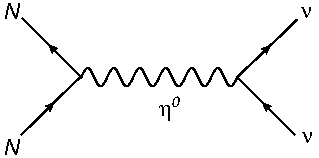
\includegraphics{imagen_1.pdf}

\section{CalcHEP comparison}

Check the result with CalcHEP. Please give the LanHEP code if necessaáry.

\section{Copyright}

\includegraphics[scale=0.5]{cc} Creative Commons Attribution-Share Alike 3.0 United States License.

%%% Local Variables:
%%% mode: latex
%%% TeX-master: "qft_samples"
%%% End:


% Radiative see saw II: Wady 0808.3340
%
\chapter{$\eta \eta \to h h$}

Author:  Wady Alexander Ríos Herrera

Proceso: \textbf{Radiative seesaw II}\\

Experimentos de reactores  de neutrinos han demostrado que los neutrinos tienen masa.


\section{Lagrangian}


El modelo considerado es una extensión del modelo estándar, el contiene SU($2$)$\times$ U($1$)$_{Y}$ de singletes $N_{i}$ y un segundo doblete de Higgs $\eta$. En adición, una simetría discreta exacta $Z_{2}$ es asumida tal que el nuevo campo son impares bajo $Z_{2}$, mientras que en el modelo estándar son pares. El lagrangiano de interacción de  Yukawa inducido por el nuevo doblete Higgs es dada por  \cite{1}
\begin{equation}
L_{Y}=\epsilon _{ab}h_{\alpha j}\bar{N}_{j}P_{L}L_{\alpha}^{a}\eta ^{b}+H.c,
\label{1}
\end{equation}
 
L son doblete de leptón izquierdo, $\alpha , j$ son indices de generación (Greek indices etiquetado sabor leptonico e,$\mu$,$\tau$) y $\epsilon _{ab}$ es el tensor antisimetrico completo.\\

A partir del lagrangiano de interacción de Yukawa se determina el langrangiano interacción escalar cuadrático  \cite{2} 

\begin{equation}
L_{I}=\lambda_{3}(\Phi^{+}\Phi)( \eta^{+}\eta)+\lambda_{2}(\Phi^{+}\eta)( \eta^{+}\Phi) \frac{\lambda _{5}}{2}(\Phi^{+}\eta + H.C)
\label{2}
\end{equation}


Donde $\Phi$ es el modelo estándar del doblete de Higgs y es solo relevante para generación de masa neutrina. Ya que $Z_{2}$ es asumida  ser  exactamente simétrica del modelo $\eta$ tiene valor esperado del vacío cero. La Física escalar de los bosones son por lo tanto $R_{e}\Phi ^{0},\eta^{\pm},\eta_{0}^{R}\equiv Re\eta_{0}, \eta_{0}^{I}\equiv Im\eta_{0} =0 $ y $Im\eta^{+} =0$.\\


para ecuación \ref{2} se tiene que 
\begin{equation}
\Phi=\begin{pmatrix}
0 & \frac{h+v}{\sqrt{2}}
\end{pmatrix}, \ \eta= \begin{pmatrix}
\eta^{+} & \\
\eta_{0} & 
\end{pmatrix} 
\label{2.1}
\end{equation}

donde $h$ y $v$ son parámetros reales por tanto $\Phi =\Phi ^{+}$


Remplazando \ref{2.1} y las partes reales de $\eta$ el lagrangiano \ref{2} se determina el termina el termino relevante

\begin{equation*}
L_{I}=\lambda_{l} \left[\begin{pmatrix}
0 & \frac{h+v}{\sqrt{2}}
\end{pmatrix}\begin{pmatrix}
\eta^{+} & \\
\eta_{0} & 
\end{pmatrix}\right]^{2}= \lambda_{l}\left[0\eta^{+}+\left( \frac{h+v}{\sqrt{2}}\right)\eta_{0}\right]^{2}
\end{equation*}
\begin{equation*}
=\lambda_{l}(h+v)^{2}(\eta_{0})^{2}=\lambda_{l}(h^{2}+2hv+v^{2})(\eta_{0})^{2}
\end{equation*}
\begin{equation}
=\underbrace{\lambda_{l}h^{2}\eta_{0}^{2}}_{\star}+2\lambda_{l}hv\eta_{0}^{2}+\lambda_{l}v^{2}\eta_{0}^{2}, 
\label{3}
\end{equation}

Con 
\begin{equation}
\lambda_{l}=\frac{\lambda _{3}+\lambda _{4}+\lambda _{5}}{2}
\end{equation}

donde el termino relevante de la expresión \ref{3} es denotado con $\star$, ya que este genera el siguiente proceso 

\begin{figure*}[htb]
    \centering
    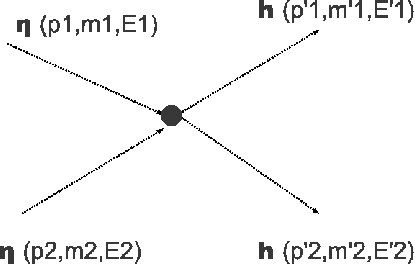
\includegraphics[width=0.5\textwidth]{1}%(eps preferiblemente)
    \caption[electrones]{Proceso donde dos etas se destruyen y se crean dos Higgs}
    \label{fi}
\end{figure*}
 



Por tanto el lagrangiano de interés es
\begin{equation}
L_{i}=\lambda_{l}h^{2}\eta_{0}^{2}
\label{4}
\end{equation}










\section{S-matriz}
 El orden a calcular la matriz $S$ es de orden uno ya que solo tenemos un termino de interacción \ref{4} el cual  determina el proceso de figuara \ref{fi}.\\
 Consideremos el proceso de la figura \ref{fi} donde $\eta(p_{1})\eta(p_{2})$ decae a un par de $h(p_{1}^{'})h(p_{2}^{'})$.
 El elemento de matriz $S_{fi}^{1}$ entre el estado inicial  y el estado final es 
 
 \begin{equation}
S_{fi}^{(1)}=-\lambda_{l}\int d^{4}x\bra{h(p_{1}^{'})h(p_{2}^{'})}h^{2}\eta_{0}^{2}\ket{\eta(p_{1})\eta(p_{2})}, 
 \label{5}
 \end{equation}
 
 sabemos que
 
 \begin{equation}
\eta_{0}=\eta_{+}+\eta_{-}=\frac{1}{\sqrt{2E_{p}V}}\left[ae^{-ip.x}+a^{+}e^{ip.x}\right]
 \label{6}
 \end{equation}

\begin{equation}
h=h_{+}+h_{-}=\frac{1}{\sqrt{2E_{p}V}}\left[ae^{-ip.x}+a^{+}e^{ip.x}\right]
 \label{7}
 \end{equation}


Por lo tanto
\begin{equation*}
h^{2}=\left(h_{+}+h_{-}\right)^{2}=(h_{+}+h_{-})(h_{+}+h_{-})
\end{equation*}
 \begin{equation}
=h_{+}h_{+}+h_{+}h_{-}+h_{-}h_{+}+h_{-}h_{-}
 \label{8}
 \end{equation}

\begin{equation*}
\eta_{0}^{2}=\left(\eta_{+}+\eta_{-}\right)^{2}=(\eta_{+}+\eta_{-})(\eta_{+}+\eta_{-})
\end{equation*}
\begin{equation}
=\eta_{+}\eta_{+}+\eta_{+}\eta_{-}+\eta_{-}\eta_{+}+\eta_{-}\eta_{-}
\label{9}
\end{equation}

El termino $\frac{1}{\sqrt{2E_{p}V}}$ de la expresión \ref{6} y \ref{7} es de normalización.\\

Calculemos  el termino $h^{2}\eta_{0}^{2}$:
\begin{equation*}
h^{2}\eta_{0}^{2}=(h_{+}h_{+}+h_{+}h_{-}+h_{-}h_{+}+h_{-}h_{-})(\eta_{+}\eta_{+}+\eta_{+}\eta_{-}+\eta_{-}\eta_{+}+\eta_{-}\eta_{-})
\end{equation*}
\begin{equation*}
=h_{+}h_{+}\eta_{+}\eta_{+}+h_{+}h_{+}\eta_{+}\eta_{-}+h_{+}h_{+}\eta_{-}\eta_{+}+h_{+}h_{+}\eta_{-}\eta_{-}+
\end{equation*}
\begin{equation*}
h_{+}h_{-}\eta_{+}\eta_{+}+h_{+}h_{-}\eta_{+}\eta_{-}+h_{+}h_{-}\eta_{-}\eta_{+}+h_{+}h_{-}\eta_{-}\eta_{-}+
\end{equation*}
\begin{equation*}
h_{-}h_{+}\eta_{+}\eta_{+}+h_{-}h_{+}\eta_{+}\eta_{-}+h_{-}h_{+}\eta_{-}\eta_{+}+h_{-}h_{+}\eta_{-}\eta_{-}+
\end{equation*}
\begin{equation}
h_{-}h_{-}\eta_{+}\eta_{+}+h_{-}h_{-}\eta_{+}\eta_{-}+h_{-}h_{-}\eta_{-}\eta_{+}+h_{-}h_{-}\eta_{-}\eta_{-}
\label{10}
\end{equation}
 Por otro lado  sabemos que 
 
 \begin{equation}
 h_{+}\ket{h}=\frac{1}{\sqrt{2E_{p}V}}e^{-ip.x}\ket0 ,\ h_{-}\ket{h}=\frac{1}{\sqrt{2E_{p}V}}e^{ip.x}\ket{1_{h}}
 \label{11}
 \end{equation}
 \begin{equation}
 \bra h h_{-}=\frac{1}{\sqrt{2E_{p}V}}e^{ip.x}\bra{0} ,\ \bra h h_{+}=\frac{1}{\sqrt{2E_{p}V}}e^{-ip.x}\bra{1_{h}}
 \label{12}
 \end{equation}


\begin{equation}
 \eta_{+}\ket{\eta}=\frac{1}{\sqrt{2E_{p}V}}e^{-ip.x}\ket0 ,\ \eta_{-}\ket{\eta}=\frac{1}{\sqrt{2E_{p}V}}e^{ip.x}\ket{1_{\eta}}
 \label{13}
 \end{equation}
 \begin{equation}
 \bra \eta \eta_{-}=\frac{1}{\sqrt{2E_{p}V}}e^{ip.x}\bra{0} ,\ \bra \eta \eta_{+}=\frac{1}{\sqrt{2E_{p}V}}e^{-ip.x}\bra {1_{\eta}}
 \label{14}
 \end{equation}
 
 y
 
 \begin{equation}
\bra{h(p_{1}^{'})h(p_{2}^{'})}h_{+}h_{+}=\frac{1}{\sqrt{2E_{p_{1}^{'}}V}}\frac{1}{\sqrt{2E_{p_{2}^{'}}V}}e^{-ip_{1}^{'}.x}e^{-ip_{2}^{'}.x}\bra{1_{h}1_{h}}
 \label{15}
 \end{equation}
\begin{equation}
\bra{h(p_{1}^{'})h(p_{2}^{'})}h_{+}h_{-}=\frac{1}{\sqrt{2E_{p_{1}^{'}}V}}\frac{1}{\sqrt{2E_{p_{2}^{'}}V}}e^{-ip_{1}^{'}.x}e^{ip_{2}^{'}.x}\bra{1_{h}0}
 \label{16}
 \end{equation}
\begin{equation}
\bra{h(p_{1}^{'})h(p_{2}^{'})}h_{-}h_{+}=\frac{1}{\sqrt{2E_{p_{1}^{'}}V}}\frac{1}{\sqrt{2E_{p_{2}^{'}}V}}e^{ip_{1}^{'}.x}e^{-ip_{2}^{'}.x}\bra{01_{h}}
 \label{17}
 \end{equation}
\begin{equation}
\bra{h(p_{1}^{'})h(p_{2}^{'})}h_{-}h_{-}=\frac{1}{\sqrt{2E_{p_{1}^{'}}V}}\frac{1}{\sqrt{2E_{p_{2}^{'}}V}}e^{ip_{1}^{'}.x}e^{ip_{2}^{'}.x}\bra{00}
 \label{18}
 \end{equation}

\begin{equation}
\eta_{+}\eta_{+}\ket{\eta(p_{1})\eta(p_{2})}=\frac{1}{\sqrt{2E_{p_{1}}V}}\frac{1}{\sqrt{2E_{p_{2}}V}}e^{-ip_{1}.x}e^{-ip_{2}.x}\ket{00}
 \label{19}
 \end{equation}


\begin{equation}
\eta_{+}\eta_{-}\ket{\eta(p_{1})\eta(p_{2})}=\frac{1}{\sqrt{2E_{p_{1}}V}}\frac{1}{\sqrt{2E_{p_{2}}V}}e^{-ip_{1}.x}e^{ip_{2}.x}\ket{01_{\eta}}
 \label{20}
 \end{equation}
\begin{equation}
\eta_{-}\eta_{+}\ket{\eta(p_{1})\eta(p_{2})}=\frac{1}{\sqrt{2E_{p_{1}}V}}\frac{1}{\sqrt{2E_{p_{2}}V}}e^{ip_{1}.x}e^{-ip_{2}.x}\ket{1_{\eta}0}
 \label{21}
 \end{equation}
\begin{equation}
\eta_{-}\eta_{-}\ket{\eta(p_{1})\eta(p_{2})}=\frac{1}{\sqrt{2E_{p_{1}}V}}\frac{1}{\sqrt{2E_{p_{2}}V}}e^{ip_{1}.x}e^{ip_{2}.x}\ket{1_{\eta}1_{\eta}}
 \label{22}
 \end{equation}

Por tanto san duchando el termino $h^{2}\eta_{0}^{2}$ con las relaciones desde \ref{15} hasta \ref{22} el termino que sobrevive es


\begin{equation*}
\bra{h(p_{1}^{'})h(p_{2}^{'})}h^{2}\eta_{0}^{2}\ket{\eta(p_{1})\eta(p_{2})}=\bra{h(p_{1}^{'})h(p_{2}^{'})}h_{-}h_{-}\eta_{+}\eta_{+}\ket{\eta(p_{1})\eta(p_{2})}
\end{equation*}
\begin{equation}
=\frac{1}{\sqrt{2E_{p_{1}^{'}}V}}\frac{1}{\sqrt{2E_{p_{2}^{'}}V}}\frac{1}{\sqrt{2E_{p_{1}}V}}\frac{1}{\sqrt{2E_{p_{2}}V}}e^{i(p_{1}^{'}+p_{2}^{'}-p_{1}-p_{2})}\bra{00}\ket{00}
\label{23}
\end{equation}

remplazando \ref{23} en matriz $S_{fi}^{(1)}$ obtenemos

\begin{equation}
S_{fi}^{(1)}=-i\lambda_{l}\frac{1}{\sqrt{2E_{p_{1}^{'}}V}}\frac{1}{\sqrt{2E_{p_{2}^{'}}V}}\frac{1}{\sqrt{2E_{p_{1}}V}}\frac{1}{\sqrt{2E_{p_{2}}V}}\int d^{4}x e^{i(p_{1}^{'}+p_{2}^{'}-p_{1}-p_{2})}\bra{00}\ket{00}
\label{24}
\end{equation}


El valor de la integral es $(2\pi)^{4}\delta^{4}(p_{1}+p_{2}-p_{1}^{'}-p_{2}^{'})$ y $\bra{00}\ket{00}=1$ por tanto el elemento de matriz obtenido es

\begin{equation}
S_{fi}^{(1)}=-i\lambda_{l}\frac{1}{\sqrt{2E_{p_{1}^{'}}V}}\frac{1}{\sqrt{2E_{p_{2}^{'}}V}}\frac{1}{\sqrt{2E_{p_{1}}V}}\frac{1}{\sqrt{2E_{p_{2}}V}}(2\pi)^{4}\delta^{4}(p_{1}+p_{2}-p_{1}^{'}-p_{2}^{'})
\label{25}
\end{equation}



\section{Process calculation}

 De la ecuación \ref{25} la función $\delta$  es la conservación de los $4$-momentos en el proceso general, el cual es multiplicado por $(2\pi)^{4}$. Hay un factor $(2EV)^{\frac{-1}{2} }$ para cada partícula del estado inicial y del estado final de energía $E$. El restos de termino de la expresión \ref{25} el cual depende sobre la naturaleza exacta de la interacción es llamada la amplitud de Feynman, es denotada por $iM_{fi}$.\\
 Para nuestro caso  
 \begin{equation}
iM_{fi}= -i\lambda_{l}
  \label{26}
 \end{equation}
              
   Para determinar la sección eficaz de nuestro modelo se determina a partir de expresión\cite{3}
   
   \begin{equation}
\frac{d\sigma}{d\Omega}=\frac{1}{64 \small{\pi} ^{2}s}\left[\frac{(s-(m_{1}^{'}+m_{2}^{'})^{2})(s-(m_{1}^{'}-m_{2}^{'})^{2}))}{(s-(m_{1}+m_{2})^{2})(s-(m_{1}-m_{2})^{2}))}\right]^{\frac{1}{2}}\overline{\vert M_{fi}\vert^{2}}
   \label{27}
   \end{equation}            
              
     Donde $m_{1}^{'}=m_{2}^{'}=m_{h}$ es la masa del Higgs, $m_{1}=m_{2}=m_{\eta}$ es la masa del eta y  $\overline{\vert M_{fi}\vert^{2}}=\lambda_{l}$ es la amplitud de Feynman, remplazando estos términos en la expresión \ref{27} se obtiene
     
     \begin{equation}
      \frac{d\sigma}{d\Omega}=\frac{1}{64\small{\pi} ^{2}s}\left[\frac{(s-4m_{h}^{2})}{(s-4m_{\eta}^{2})}\right]^{\frac{1}{2}}\left(\lambda_{l}\right)^{2}
          \label{28}
     \end{equation}
     
     
Con $s=\sqrt{E_{1}+E_{2}}$ y $E=\sqrt{p^{2}+m^{2}}$, la integral sobre $d\Omega$ es $4\pi$ por tanto la sección eficaz es 


\begin{equation}
  \sigma=\frac{(\lambda_{l})^{2}}{64\small{\pi} s}\left[\frac{(s-4m_{h}^{2})}{(s-4m_{\eta}^{2})}\right]^{\frac{1}{2}}
  \label{29}
\end{equation}  
          
     
     
Para determinar un valor númerico de la sección eficaz tomamos los siguientes valores: $ m_{\eta}=50GeV, m_{h}=120 GeV, \lambda_{l}=0.1$ y $\sqrt{s}=1016.68GeV $, Por tanto la expresión \ref{29} que así

\begin{equation*}
\sigma=\frac{(0.1)^{2}}{64\small{\pi} (1016.68GeV)^{2}}\left[\frac{(1016.68GeV)^{2}-4(120GeV)^{2}}{(1016.68GeV)^{2}-4(50GeV)^{2}}\right]^{\frac{1}{2}}
\label{30}GeV
\end{equation*}
     \begin{equation*}
    \frac{(0.1)^{2}}{64\small{\pi} (1016.68GeV)^{2}}\left[\frac{976055.3134 (GeV)^{2}}{1023638.232(GeV)^{2}}\right]^{\frac{1}{2}}
     \end{equation*}
              
\begin{equation*}
   = \frac{(0.1)^{2}}{64\small{\pi} (1016.68GeV)^{2}}(0,9764)
     \end{equation*}   
     \begin{equation}
    =4,69\times 10^{-11}(GeV)^{-2}
     \end{equation}              
              
\section{CalcHEP comparison}
Para ser la simulación se instala los programas de LanHep y CalHep.\\
Después se baja los archivos del proceso a simular de github, nuestro archivo pertinente es la carpeta idm para nuestro sistema. Se  instala la carpeta idm  en LanHep y CalHep y se ejecuta  CalHep desde el directorio idm para iniciar la simulación.\\
Los parámetros de la simulación son $~H0,~H0->H,H$ donde se descoge el diagrama de la figura \ref{fi} luego se ingresa los parámetros de la simulación que son $\lambda_{l}=0.1, m_{\eta}=50 GeV, m_{h}=120 GeV$, momento inicial $500 GeV$ y momento final es de $500GeV$ por tanto al sección eficaz de la simulación es de $0.145983[pb]$  

\section{Copyright}

\includegraphics[scale=0.5]{cc} Creative Commons Attribution-Share Alike 3.0 United States License.

\begin{thebibliography}{9}

\bibitem{1} D. Aristizabal Sierra, Jisuke Kubo and Daijiro Suematsu, Physical Review D 79, 013001 (2009)
\bibitem{2} Ernast Ma, Physical Review D 73, 0077301(2006)
\bibitem{3} Quantum Fiel Theory, Amitabha Lahiri and Palash B. Pal

\end{thebibliography}

%%% Local Variables: 
%%% mode: latex
%%% TeX-master: "qft_samples"
%%% End: 

% Radiative see saw III: 
%
\chapter{$\eta \eta \to h h$}

Author:  Wady Alexander Ríos Herrera

Proceso: \textbf{Radiative seesaw II}\\

Experimentos de reactores  de neutrinos han demostrado que los neutrinos tienen masa.


\section{Lagrangian}


El modelo considerado es una extensión del modelo estándar, el contiene SU($2$)$\times$ U($1$)$_{Y}$ de singletes $N_{i}$ y un segundo doblete de Higgs $\eta$. En adición, una simetría discreta exacta $Z_{2}$ es asumida tal que el nuevo campo son impares bajo $Z_{2}$, mientras que en el modelo estándar son pares. El lagrangiano de interacción de  Yukawa inducido por el nuevo doblete Higgs es dada por  \cite{1}
\begin{equation}
L_{Y}=\epsilon _{ab}h_{\alpha j}\bar{N}_{j}P_{L}L_{\alpha}^{a}\eta ^{b}+H.c,
\label{1}
\end{equation}
 
L son doblete de leptón izquierdo, $\alpha , j$ son indices de generación (Greek indices etiquetado sabor leptonico e,$\mu$,$\tau$) y $\epsilon _{ab}$ es el tensor antisimetrico completo.\\

A partir del lagrangiano de interacción de Yukawa se determina el langrangiano interacción escalar cuadrático  \cite{2} 

\begin{equation}
L_{I}=\lambda_{3}(\Phi^{+}\Phi)( \eta^{+}\eta)+\lambda_{2}(\Phi^{+}\eta)( \eta^{+}\Phi) \frac{\lambda _{5}}{2}(\Phi^{+}\eta + H.C)
\label{2}
\end{equation}


Donde $\Phi$ es el modelo estándar del doblete de Higgs y es solo relevante para generación de masa neutrina. Ya que $Z_{2}$ es asumida  ser  exactamente simétrica del modelo $\eta$ tiene valor esperado del vacío cero. La Física escalar de los bosones son por lo tanto $R_{e}\Phi ^{0},\eta^{\pm},\eta_{0}^{R}\equiv Re\eta_{0}, \eta_{0}^{I}\equiv Im\eta_{0} =0 $ y $Im\eta^{+} =0$.\\


para ecuación \ref{2} se tiene que 
\begin{equation}
\Phi=\begin{pmatrix}
0 & \frac{h+v}{\sqrt{2}}
\end{pmatrix}, \ \eta= \begin{pmatrix}
\eta^{+} & \\
\eta_{0} & 
\end{pmatrix} 
\label{2.1}
\end{equation}

donde $h$ y $v$ son parámetros reales por tanto $\Phi =\Phi ^{+}$


Remplazando \ref{2.1} y las partes reales de $\eta$ el lagrangiano \ref{2} se determina el termina el termino relevante

\begin{equation*}
L_{I}=\lambda_{l} \left[\begin{pmatrix}
0 & \frac{h+v}{\sqrt{2}}
\end{pmatrix}\begin{pmatrix}
\eta^{+} & \\
\eta_{0} & 
\end{pmatrix}\right]^{2}= \lambda_{l}\left[0\eta^{+}+\left( \frac{h+v}{\sqrt{2}}\right)\eta_{0}\right]^{2}
\end{equation*}
\begin{equation*}
=\lambda_{l}(h+v)^{2}(\eta_{0})^{2}=\lambda_{l}(h^{2}+2hv+v^{2})(\eta_{0})^{2}
\end{equation*}
\begin{equation}
=\underbrace{\lambda_{l}h^{2}\eta_{0}^{2}}_{\star}+2\lambda_{l}hv\eta_{0}^{2}+\lambda_{l}v^{2}\eta_{0}^{2}, 
\label{3}
\end{equation}

Con 
\begin{equation}
\lambda_{l}=\frac{\lambda _{3}+\lambda _{4}+\lambda _{5}}{2}
\end{equation}

donde el termino relevante de la expresión \ref{3} es denotado con $\star$, ya que este genera el siguiente proceso 

\begin{figure*}[htb]
    \centering
    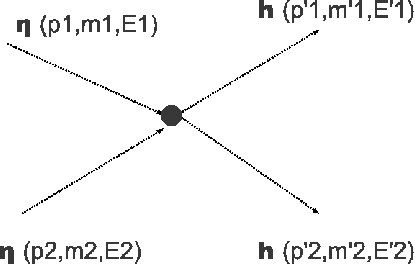
\includegraphics[width=0.5\textwidth]{1}%(eps preferiblemente)
    \caption[electrones]{Proceso donde dos etas se destruyen y se crean dos Higgs}
    \label{fi}
\end{figure*}
 



Por tanto el lagrangiano de interés es
\begin{equation}
L_{i}=\lambda_{l}h^{2}\eta_{0}^{2}
\label{4}
\end{equation}










\section{S-matriz}
 El orden a calcular la matriz $S$ es de orden uno ya que solo tenemos un termino de interacción \ref{4} el cual  determina el proceso de figuara \ref{fi}.\\
 Consideremos el proceso de la figura \ref{fi} donde $\eta(p_{1})\eta(p_{2})$ decae a un par de $h(p_{1}^{'})h(p_{2}^{'})$.
 El elemento de matriz $S_{fi}^{1}$ entre el estado inicial  y el estado final es 
 
 \begin{equation}
S_{fi}^{(1)}=-\lambda_{l}\int d^{4}x\bra{h(p_{1}^{'})h(p_{2}^{'})}h^{2}\eta_{0}^{2}\ket{\eta(p_{1})\eta(p_{2})}, 
 \label{5}
 \end{equation}
 
 sabemos que
 
 \begin{equation}
\eta_{0}=\eta_{+}+\eta_{-}=\frac{1}{\sqrt{2E_{p}V}}\left[ae^{-ip.x}+a^{+}e^{ip.x}\right]
 \label{6}
 \end{equation}

\begin{equation}
h=h_{+}+h_{-}=\frac{1}{\sqrt{2E_{p}V}}\left[ae^{-ip.x}+a^{+}e^{ip.x}\right]
 \label{7}
 \end{equation}


Por lo tanto
\begin{equation*}
h^{2}=\left(h_{+}+h_{-}\right)^{2}=(h_{+}+h_{-})(h_{+}+h_{-})
\end{equation*}
 \begin{equation}
=h_{+}h_{+}+h_{+}h_{-}+h_{-}h_{+}+h_{-}h_{-}
 \label{8}
 \end{equation}

\begin{equation*}
\eta_{0}^{2}=\left(\eta_{+}+\eta_{-}\right)^{2}=(\eta_{+}+\eta_{-})(\eta_{+}+\eta_{-})
\end{equation*}
\begin{equation}
=\eta_{+}\eta_{+}+\eta_{+}\eta_{-}+\eta_{-}\eta_{+}+\eta_{-}\eta_{-}
\label{9}
\end{equation}

El termino $\frac{1}{\sqrt{2E_{p}V}}$ de la expresión \ref{6} y \ref{7} es de normalización.\\

Calculemos  el termino $h^{2}\eta_{0}^{2}$:
\begin{equation*}
h^{2}\eta_{0}^{2}=(h_{+}h_{+}+h_{+}h_{-}+h_{-}h_{+}+h_{-}h_{-})(\eta_{+}\eta_{+}+\eta_{+}\eta_{-}+\eta_{-}\eta_{+}+\eta_{-}\eta_{-})
\end{equation*}
\begin{equation*}
=h_{+}h_{+}\eta_{+}\eta_{+}+h_{+}h_{+}\eta_{+}\eta_{-}+h_{+}h_{+}\eta_{-}\eta_{+}+h_{+}h_{+}\eta_{-}\eta_{-}+
\end{equation*}
\begin{equation*}
h_{+}h_{-}\eta_{+}\eta_{+}+h_{+}h_{-}\eta_{+}\eta_{-}+h_{+}h_{-}\eta_{-}\eta_{+}+h_{+}h_{-}\eta_{-}\eta_{-}+
\end{equation*}
\begin{equation*}
h_{-}h_{+}\eta_{+}\eta_{+}+h_{-}h_{+}\eta_{+}\eta_{-}+h_{-}h_{+}\eta_{-}\eta_{+}+h_{-}h_{+}\eta_{-}\eta_{-}+
\end{equation*}
\begin{equation}
h_{-}h_{-}\eta_{+}\eta_{+}+h_{-}h_{-}\eta_{+}\eta_{-}+h_{-}h_{-}\eta_{-}\eta_{+}+h_{-}h_{-}\eta_{-}\eta_{-}
\label{10}
\end{equation}
 Por otro lado  sabemos que 
 
 \begin{equation}
 h_{+}\ket{h}=\frac{1}{\sqrt{2E_{p}V}}e^{-ip.x}\ket0 ,\ h_{-}\ket{h}=\frac{1}{\sqrt{2E_{p}V}}e^{ip.x}\ket{1_{h}}
 \label{11}
 \end{equation}
 \begin{equation}
 \bra h h_{-}=\frac{1}{\sqrt{2E_{p}V}}e^{ip.x}\bra{0} ,\ \bra h h_{+}=\frac{1}{\sqrt{2E_{p}V}}e^{-ip.x}\bra{1_{h}}
 \label{12}
 \end{equation}


\begin{equation}
 \eta_{+}\ket{\eta}=\frac{1}{\sqrt{2E_{p}V}}e^{-ip.x}\ket0 ,\ \eta_{-}\ket{\eta}=\frac{1}{\sqrt{2E_{p}V}}e^{ip.x}\ket{1_{\eta}}
 \label{13}
 \end{equation}
 \begin{equation}
 \bra \eta \eta_{-}=\frac{1}{\sqrt{2E_{p}V}}e^{ip.x}\bra{0} ,\ \bra \eta \eta_{+}=\frac{1}{\sqrt{2E_{p}V}}e^{-ip.x}\bra {1_{\eta}}
 \label{14}
 \end{equation}
 
 y
 
 \begin{equation}
\bra{h(p_{1}^{'})h(p_{2}^{'})}h_{+}h_{+}=\frac{1}{\sqrt{2E_{p_{1}^{'}}V}}\frac{1}{\sqrt{2E_{p_{2}^{'}}V}}e^{-ip_{1}^{'}.x}e^{-ip_{2}^{'}.x}\bra{1_{h}1_{h}}
 \label{15}
 \end{equation}
\begin{equation}
\bra{h(p_{1}^{'})h(p_{2}^{'})}h_{+}h_{-}=\frac{1}{\sqrt{2E_{p_{1}^{'}}V}}\frac{1}{\sqrt{2E_{p_{2}^{'}}V}}e^{-ip_{1}^{'}.x}e^{ip_{2}^{'}.x}\bra{1_{h}0}
 \label{16}
 \end{equation}
\begin{equation}
\bra{h(p_{1}^{'})h(p_{2}^{'})}h_{-}h_{+}=\frac{1}{\sqrt{2E_{p_{1}^{'}}V}}\frac{1}{\sqrt{2E_{p_{2}^{'}}V}}e^{ip_{1}^{'}.x}e^{-ip_{2}^{'}.x}\bra{01_{h}}
 \label{17}
 \end{equation}
\begin{equation}
\bra{h(p_{1}^{'})h(p_{2}^{'})}h_{-}h_{-}=\frac{1}{\sqrt{2E_{p_{1}^{'}}V}}\frac{1}{\sqrt{2E_{p_{2}^{'}}V}}e^{ip_{1}^{'}.x}e^{ip_{2}^{'}.x}\bra{00}
 \label{18}
 \end{equation}

\begin{equation}
\eta_{+}\eta_{+}\ket{\eta(p_{1})\eta(p_{2})}=\frac{1}{\sqrt{2E_{p_{1}}V}}\frac{1}{\sqrt{2E_{p_{2}}V}}e^{-ip_{1}.x}e^{-ip_{2}.x}\ket{00}
 \label{19}
 \end{equation}


\begin{equation}
\eta_{+}\eta_{-}\ket{\eta(p_{1})\eta(p_{2})}=\frac{1}{\sqrt{2E_{p_{1}}V}}\frac{1}{\sqrt{2E_{p_{2}}V}}e^{-ip_{1}.x}e^{ip_{2}.x}\ket{01_{\eta}}
 \label{20}
 \end{equation}
\begin{equation}
\eta_{-}\eta_{+}\ket{\eta(p_{1})\eta(p_{2})}=\frac{1}{\sqrt{2E_{p_{1}}V}}\frac{1}{\sqrt{2E_{p_{2}}V}}e^{ip_{1}.x}e^{-ip_{2}.x}\ket{1_{\eta}0}
 \label{21}
 \end{equation}
\begin{equation}
\eta_{-}\eta_{-}\ket{\eta(p_{1})\eta(p_{2})}=\frac{1}{\sqrt{2E_{p_{1}}V}}\frac{1}{\sqrt{2E_{p_{2}}V}}e^{ip_{1}.x}e^{ip_{2}.x}\ket{1_{\eta}1_{\eta}}
 \label{22}
 \end{equation}

Por tanto san duchando el termino $h^{2}\eta_{0}^{2}$ con las relaciones desde \ref{15} hasta \ref{22} el termino que sobrevive es


\begin{equation*}
\bra{h(p_{1}^{'})h(p_{2}^{'})}h^{2}\eta_{0}^{2}\ket{\eta(p_{1})\eta(p_{2})}=\bra{h(p_{1}^{'})h(p_{2}^{'})}h_{-}h_{-}\eta_{+}\eta_{+}\ket{\eta(p_{1})\eta(p_{2})}
\end{equation*}
\begin{equation}
=\frac{1}{\sqrt{2E_{p_{1}^{'}}V}}\frac{1}{\sqrt{2E_{p_{2}^{'}}V}}\frac{1}{\sqrt{2E_{p_{1}}V}}\frac{1}{\sqrt{2E_{p_{2}}V}}e^{i(p_{1}^{'}+p_{2}^{'}-p_{1}-p_{2})}\bra{00}\ket{00}
\label{23}
\end{equation}

remplazando \ref{23} en matriz $S_{fi}^{(1)}$ obtenemos

\begin{equation}
S_{fi}^{(1)}=-i\lambda_{l}\frac{1}{\sqrt{2E_{p_{1}^{'}}V}}\frac{1}{\sqrt{2E_{p_{2}^{'}}V}}\frac{1}{\sqrt{2E_{p_{1}}V}}\frac{1}{\sqrt{2E_{p_{2}}V}}\int d^{4}x e^{i(p_{1}^{'}+p_{2}^{'}-p_{1}-p_{2})}\bra{00}\ket{00}
\label{24}
\end{equation}


El valor de la integral es $(2\pi)^{4}\delta^{4}(p_{1}+p_{2}-p_{1}^{'}-p_{2}^{'})$ y $\bra{00}\ket{00}=1$ por tanto el elemento de matriz obtenido es

\begin{equation}
S_{fi}^{(1)}=-i\lambda_{l}\frac{1}{\sqrt{2E_{p_{1}^{'}}V}}\frac{1}{\sqrt{2E_{p_{2}^{'}}V}}\frac{1}{\sqrt{2E_{p_{1}}V}}\frac{1}{\sqrt{2E_{p_{2}}V}}(2\pi)^{4}\delta^{4}(p_{1}+p_{2}-p_{1}^{'}-p_{2}^{'})
\label{25}
\end{equation}



\section{Process calculation}

 De la ecuación \ref{25} la función $\delta$  es la conservación de los $4$-momentos en el proceso general, el cual es multiplicado por $(2\pi)^{4}$. Hay un factor $(2EV)^{\frac{-1}{2} }$ para cada partícula del estado inicial y del estado final de energía $E$. El restos de termino de la expresión \ref{25} el cual depende sobre la naturaleza exacta de la interacción es llamada la amplitud de Feynman, es denotada por $iM_{fi}$.\\
 Para nuestro caso  
 \begin{equation}
iM_{fi}= -i\lambda_{l}
  \label{26}
 \end{equation}
              
   Para determinar la sección eficaz de nuestro modelo se determina a partir de expresión\cite{3}
   
   \begin{equation}
\frac{d\sigma}{d\Omega}=\frac{1}{64 \small{\pi} ^{2}s}\left[\frac{(s-(m_{1}^{'}+m_{2}^{'})^{2})(s-(m_{1}^{'}-m_{2}^{'})^{2}))}{(s-(m_{1}+m_{2})^{2})(s-(m_{1}-m_{2})^{2}))}\right]^{\frac{1}{2}}\overline{\vert M_{fi}\vert^{2}}
   \label{27}
   \end{equation}            
              
     Donde $m_{1}^{'}=m_{2}^{'}=m_{h}$ es la masa del Higgs, $m_{1}=m_{2}=m_{\eta}$ es la masa del eta y  $\overline{\vert M_{fi}\vert^{2}}=\lambda_{l}$ es la amplitud de Feynman, remplazando estos términos en la expresión \ref{27} se obtiene
     
     \begin{equation}
      \frac{d\sigma}{d\Omega}=\frac{1}{64\small{\pi} ^{2}s}\left[\frac{(s-4m_{h}^{2})}{(s-4m_{\eta}^{2})}\right]^{\frac{1}{2}}\left(\lambda_{l}\right)^{2}
          \label{28}
     \end{equation}
     
     
Con $s=\sqrt{E_{1}+E_{2}}$ y $E=\sqrt{p^{2}+m^{2}}$, la integral sobre $d\Omega$ es $4\pi$ por tanto la sección eficaz es 


\begin{equation}
  \sigma=\frac{(\lambda_{l})^{2}}{64\small{\pi} s}\left[\frac{(s-4m_{h}^{2})}{(s-4m_{\eta}^{2})}\right]^{\frac{1}{2}}
  \label{29}
\end{equation}  
          
     
     
Para determinar un valor númerico de la sección eficaz tomamos los siguientes valores: $ m_{\eta}=50GeV, m_{h}=120 GeV, \lambda_{l}=0.1$ y $\sqrt{s}=1016.68GeV $, Por tanto la expresión \ref{29} que así

\begin{equation*}
\sigma=\frac{(0.1)^{2}}{64\small{\pi} (1016.68GeV)^{2}}\left[\frac{(1016.68GeV)^{2}-4(120GeV)^{2}}{(1016.68GeV)^{2}-4(50GeV)^{2}}\right]^{\frac{1}{2}}
\label{30}GeV
\end{equation*}
     \begin{equation*}
    \frac{(0.1)^{2}}{64\small{\pi} (1016.68GeV)^{2}}\left[\frac{976055.3134 (GeV)^{2}}{1023638.232(GeV)^{2}}\right]^{\frac{1}{2}}
     \end{equation*}
              
\begin{equation*}
   = \frac{(0.1)^{2}}{64\small{\pi} (1016.68GeV)^{2}}(0,9764)
     \end{equation*}   
     \begin{equation}
    =4,69\times 10^{-11}(GeV)^{-2}
     \end{equation}              
              
\section{CalcHEP comparison}
Para ser la simulación se instala los programas de LanHep y CalHep.\\
Después se baja los archivos del proceso a simular de github, nuestro archivo pertinente es la carpeta idm para nuestro sistema. Se  instala la carpeta idm  en LanHep y CalHep y se ejecuta  CalHep desde el directorio idm para iniciar la simulación.\\
Los parámetros de la simulación son $~H0,~H0->H,H$ donde se descoge el diagrama de la figura \ref{fi} luego se ingresa los parámetros de la simulación que son $\lambda_{l}=0.1, m_{\eta}=50 GeV, m_{h}=120 GeV$, momento inicial $500 GeV$ y momento final es de $500GeV$ por tanto al sección eficaz de la simulación es de $0.145983[pb]$  

\section{Copyright}

\includegraphics[scale=0.5]{cc} Creative Commons Attribution-Share Alike 3.0 United States License.

\begin{thebibliography}{9}

\bibitem{1} D. Aristizabal Sierra, Jisuke Kubo and Daijiro Suematsu, Physical Review D 79, 013001 (2009)
\bibitem{2} Ernast Ma, Physical Review D 73, 0077301(2006)
\bibitem{3} Quantum Fiel Theory, Amitabha Lahiri and Palash B. Pal

\end{thebibliography}

%%% Local Variables: 
%%% mode: latex
%%% TeX-master: "qft_samples"
%%% End: 

% zee model I: Andrés hep-ph/0604012
%
\chapter{$\eta \eta \to h h$}

Author:  Wady Alexander Ríos Herrera

Proceso: \textbf{Radiative seesaw II}\\

Experimentos de reactores  de neutrinos han demostrado que los neutrinos tienen masa.


\section{Lagrangian}


El modelo considerado es una extensión del modelo estándar, el contiene SU($2$)$\times$ U($1$)$_{Y}$ de singletes $N_{i}$ y un segundo doblete de Higgs $\eta$. En adición, una simetría discreta exacta $Z_{2}$ es asumida tal que el nuevo campo son impares bajo $Z_{2}$, mientras que en el modelo estándar son pares. El lagrangiano de interacción de  Yukawa inducido por el nuevo doblete Higgs es dada por  \cite{1}
\begin{equation}
L_{Y}=\epsilon _{ab}h_{\alpha j}\bar{N}_{j}P_{L}L_{\alpha}^{a}\eta ^{b}+H.c,
\label{1}
\end{equation}
 
L son doblete de leptón izquierdo, $\alpha , j$ son indices de generación (Greek indices etiquetado sabor leptonico e,$\mu$,$\tau$) y $\epsilon _{ab}$ es el tensor antisimetrico completo.\\

A partir del lagrangiano de interacción de Yukawa se determina el langrangiano interacción escalar cuadrático  \cite{2} 

\begin{equation}
L_{I}=\lambda_{3}(\Phi^{+}\Phi)( \eta^{+}\eta)+\lambda_{2}(\Phi^{+}\eta)( \eta^{+}\Phi) \frac{\lambda _{5}}{2}(\Phi^{+}\eta + H.C)
\label{2}
\end{equation}


Donde $\Phi$ es el modelo estándar del doblete de Higgs y es solo relevante para generación de masa neutrina. Ya que $Z_{2}$ es asumida  ser  exactamente simétrica del modelo $\eta$ tiene valor esperado del vacío cero. La Física escalar de los bosones son por lo tanto $R_{e}\Phi ^{0},\eta^{\pm},\eta_{0}^{R}\equiv Re\eta_{0}, \eta_{0}^{I}\equiv Im\eta_{0} =0 $ y $Im\eta^{+} =0$.\\


para ecuación \ref{2} se tiene que 
\begin{equation}
\Phi=\begin{pmatrix}
0 & \frac{h+v}{\sqrt{2}}
\end{pmatrix}, \ \eta= \begin{pmatrix}
\eta^{+} & \\
\eta_{0} & 
\end{pmatrix} 
\label{2.1}
\end{equation}

donde $h$ y $v$ son parámetros reales por tanto $\Phi =\Phi ^{+}$


Remplazando \ref{2.1} y las partes reales de $\eta$ el lagrangiano \ref{2} se determina el termina el termino relevante

\begin{equation*}
L_{I}=\lambda_{l} \left[\begin{pmatrix}
0 & \frac{h+v}{\sqrt{2}}
\end{pmatrix}\begin{pmatrix}
\eta^{+} & \\
\eta_{0} & 
\end{pmatrix}\right]^{2}= \lambda_{l}\left[0\eta^{+}+\left( \frac{h+v}{\sqrt{2}}\right)\eta_{0}\right]^{2}
\end{equation*}
\begin{equation*}
=\lambda_{l}(h+v)^{2}(\eta_{0})^{2}=\lambda_{l}(h^{2}+2hv+v^{2})(\eta_{0})^{2}
\end{equation*}
\begin{equation}
=\underbrace{\lambda_{l}h^{2}\eta_{0}^{2}}_{\star}+2\lambda_{l}hv\eta_{0}^{2}+\lambda_{l}v^{2}\eta_{0}^{2}, 
\label{3}
\end{equation}

Con 
\begin{equation}
\lambda_{l}=\frac{\lambda _{3}+\lambda _{4}+\lambda _{5}}{2}
\end{equation}

donde el termino relevante de la expresión \ref{3} es denotado con $\star$, ya que este genera el siguiente proceso 

\begin{figure*}[htb]
    \centering
    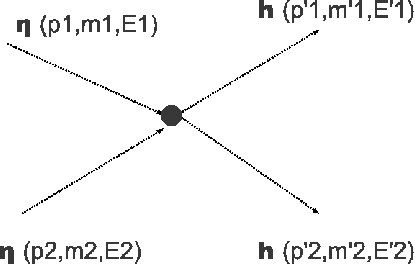
\includegraphics[width=0.5\textwidth]{1}%(eps preferiblemente)
    \caption[electrones]{Proceso donde dos etas se destruyen y se crean dos Higgs}
    \label{fi}
\end{figure*}
 



Por tanto el lagrangiano de interés es
\begin{equation}
L_{i}=\lambda_{l}h^{2}\eta_{0}^{2}
\label{4}
\end{equation}










\section{S-matriz}
 El orden a calcular la matriz $S$ es de orden uno ya que solo tenemos un termino de interacción \ref{4} el cual  determina el proceso de figuara \ref{fi}.\\
 Consideremos el proceso de la figura \ref{fi} donde $\eta(p_{1})\eta(p_{2})$ decae a un par de $h(p_{1}^{'})h(p_{2}^{'})$.
 El elemento de matriz $S_{fi}^{1}$ entre el estado inicial  y el estado final es 
 
 \begin{equation}
S_{fi}^{(1)}=-\lambda_{l}\int d^{4}x\bra{h(p_{1}^{'})h(p_{2}^{'})}h^{2}\eta_{0}^{2}\ket{\eta(p_{1})\eta(p_{2})}, 
 \label{5}
 \end{equation}
 
 sabemos que
 
 \begin{equation}
\eta_{0}=\eta_{+}+\eta_{-}=\frac{1}{\sqrt{2E_{p}V}}\left[ae^{-ip.x}+a^{+}e^{ip.x}\right]
 \label{6}
 \end{equation}

\begin{equation}
h=h_{+}+h_{-}=\frac{1}{\sqrt{2E_{p}V}}\left[ae^{-ip.x}+a^{+}e^{ip.x}\right]
 \label{7}
 \end{equation}


Por lo tanto
\begin{equation*}
h^{2}=\left(h_{+}+h_{-}\right)^{2}=(h_{+}+h_{-})(h_{+}+h_{-})
\end{equation*}
 \begin{equation}
=h_{+}h_{+}+h_{+}h_{-}+h_{-}h_{+}+h_{-}h_{-}
 \label{8}
 \end{equation}

\begin{equation*}
\eta_{0}^{2}=\left(\eta_{+}+\eta_{-}\right)^{2}=(\eta_{+}+\eta_{-})(\eta_{+}+\eta_{-})
\end{equation*}
\begin{equation}
=\eta_{+}\eta_{+}+\eta_{+}\eta_{-}+\eta_{-}\eta_{+}+\eta_{-}\eta_{-}
\label{9}
\end{equation}

El termino $\frac{1}{\sqrt{2E_{p}V}}$ de la expresión \ref{6} y \ref{7} es de normalización.\\

Calculemos  el termino $h^{2}\eta_{0}^{2}$:
\begin{equation*}
h^{2}\eta_{0}^{2}=(h_{+}h_{+}+h_{+}h_{-}+h_{-}h_{+}+h_{-}h_{-})(\eta_{+}\eta_{+}+\eta_{+}\eta_{-}+\eta_{-}\eta_{+}+\eta_{-}\eta_{-})
\end{equation*}
\begin{equation*}
=h_{+}h_{+}\eta_{+}\eta_{+}+h_{+}h_{+}\eta_{+}\eta_{-}+h_{+}h_{+}\eta_{-}\eta_{+}+h_{+}h_{+}\eta_{-}\eta_{-}+
\end{equation*}
\begin{equation*}
h_{+}h_{-}\eta_{+}\eta_{+}+h_{+}h_{-}\eta_{+}\eta_{-}+h_{+}h_{-}\eta_{-}\eta_{+}+h_{+}h_{-}\eta_{-}\eta_{-}+
\end{equation*}
\begin{equation*}
h_{-}h_{+}\eta_{+}\eta_{+}+h_{-}h_{+}\eta_{+}\eta_{-}+h_{-}h_{+}\eta_{-}\eta_{+}+h_{-}h_{+}\eta_{-}\eta_{-}+
\end{equation*}
\begin{equation}
h_{-}h_{-}\eta_{+}\eta_{+}+h_{-}h_{-}\eta_{+}\eta_{-}+h_{-}h_{-}\eta_{-}\eta_{+}+h_{-}h_{-}\eta_{-}\eta_{-}
\label{10}
\end{equation}
 Por otro lado  sabemos que 
 
 \begin{equation}
 h_{+}\ket{h}=\frac{1}{\sqrt{2E_{p}V}}e^{-ip.x}\ket0 ,\ h_{-}\ket{h}=\frac{1}{\sqrt{2E_{p}V}}e^{ip.x}\ket{1_{h}}
 \label{11}
 \end{equation}
 \begin{equation}
 \bra h h_{-}=\frac{1}{\sqrt{2E_{p}V}}e^{ip.x}\bra{0} ,\ \bra h h_{+}=\frac{1}{\sqrt{2E_{p}V}}e^{-ip.x}\bra{1_{h}}
 \label{12}
 \end{equation}


\begin{equation}
 \eta_{+}\ket{\eta}=\frac{1}{\sqrt{2E_{p}V}}e^{-ip.x}\ket0 ,\ \eta_{-}\ket{\eta}=\frac{1}{\sqrt{2E_{p}V}}e^{ip.x}\ket{1_{\eta}}
 \label{13}
 \end{equation}
 \begin{equation}
 \bra \eta \eta_{-}=\frac{1}{\sqrt{2E_{p}V}}e^{ip.x}\bra{0} ,\ \bra \eta \eta_{+}=\frac{1}{\sqrt{2E_{p}V}}e^{-ip.x}\bra {1_{\eta}}
 \label{14}
 \end{equation}
 
 y
 
 \begin{equation}
\bra{h(p_{1}^{'})h(p_{2}^{'})}h_{+}h_{+}=\frac{1}{\sqrt{2E_{p_{1}^{'}}V}}\frac{1}{\sqrt{2E_{p_{2}^{'}}V}}e^{-ip_{1}^{'}.x}e^{-ip_{2}^{'}.x}\bra{1_{h}1_{h}}
 \label{15}
 \end{equation}
\begin{equation}
\bra{h(p_{1}^{'})h(p_{2}^{'})}h_{+}h_{-}=\frac{1}{\sqrt{2E_{p_{1}^{'}}V}}\frac{1}{\sqrt{2E_{p_{2}^{'}}V}}e^{-ip_{1}^{'}.x}e^{ip_{2}^{'}.x}\bra{1_{h}0}
 \label{16}
 \end{equation}
\begin{equation}
\bra{h(p_{1}^{'})h(p_{2}^{'})}h_{-}h_{+}=\frac{1}{\sqrt{2E_{p_{1}^{'}}V}}\frac{1}{\sqrt{2E_{p_{2}^{'}}V}}e^{ip_{1}^{'}.x}e^{-ip_{2}^{'}.x}\bra{01_{h}}
 \label{17}
 \end{equation}
\begin{equation}
\bra{h(p_{1}^{'})h(p_{2}^{'})}h_{-}h_{-}=\frac{1}{\sqrt{2E_{p_{1}^{'}}V}}\frac{1}{\sqrt{2E_{p_{2}^{'}}V}}e^{ip_{1}^{'}.x}e^{ip_{2}^{'}.x}\bra{00}
 \label{18}
 \end{equation}

\begin{equation}
\eta_{+}\eta_{+}\ket{\eta(p_{1})\eta(p_{2})}=\frac{1}{\sqrt{2E_{p_{1}}V}}\frac{1}{\sqrt{2E_{p_{2}}V}}e^{-ip_{1}.x}e^{-ip_{2}.x}\ket{00}
 \label{19}
 \end{equation}


\begin{equation}
\eta_{+}\eta_{-}\ket{\eta(p_{1})\eta(p_{2})}=\frac{1}{\sqrt{2E_{p_{1}}V}}\frac{1}{\sqrt{2E_{p_{2}}V}}e^{-ip_{1}.x}e^{ip_{2}.x}\ket{01_{\eta}}
 \label{20}
 \end{equation}
\begin{equation}
\eta_{-}\eta_{+}\ket{\eta(p_{1})\eta(p_{2})}=\frac{1}{\sqrt{2E_{p_{1}}V}}\frac{1}{\sqrt{2E_{p_{2}}V}}e^{ip_{1}.x}e^{-ip_{2}.x}\ket{1_{\eta}0}
 \label{21}
 \end{equation}
\begin{equation}
\eta_{-}\eta_{-}\ket{\eta(p_{1})\eta(p_{2})}=\frac{1}{\sqrt{2E_{p_{1}}V}}\frac{1}{\sqrt{2E_{p_{2}}V}}e^{ip_{1}.x}e^{ip_{2}.x}\ket{1_{\eta}1_{\eta}}
 \label{22}
 \end{equation}

Por tanto san duchando el termino $h^{2}\eta_{0}^{2}$ con las relaciones desde \ref{15} hasta \ref{22} el termino que sobrevive es


\begin{equation*}
\bra{h(p_{1}^{'})h(p_{2}^{'})}h^{2}\eta_{0}^{2}\ket{\eta(p_{1})\eta(p_{2})}=\bra{h(p_{1}^{'})h(p_{2}^{'})}h_{-}h_{-}\eta_{+}\eta_{+}\ket{\eta(p_{1})\eta(p_{2})}
\end{equation*}
\begin{equation}
=\frac{1}{\sqrt{2E_{p_{1}^{'}}V}}\frac{1}{\sqrt{2E_{p_{2}^{'}}V}}\frac{1}{\sqrt{2E_{p_{1}}V}}\frac{1}{\sqrt{2E_{p_{2}}V}}e^{i(p_{1}^{'}+p_{2}^{'}-p_{1}-p_{2})}\bra{00}\ket{00}
\label{23}
\end{equation}

remplazando \ref{23} en matriz $S_{fi}^{(1)}$ obtenemos

\begin{equation}
S_{fi}^{(1)}=-i\lambda_{l}\frac{1}{\sqrt{2E_{p_{1}^{'}}V}}\frac{1}{\sqrt{2E_{p_{2}^{'}}V}}\frac{1}{\sqrt{2E_{p_{1}}V}}\frac{1}{\sqrt{2E_{p_{2}}V}}\int d^{4}x e^{i(p_{1}^{'}+p_{2}^{'}-p_{1}-p_{2})}\bra{00}\ket{00}
\label{24}
\end{equation}


El valor de la integral es $(2\pi)^{4}\delta^{4}(p_{1}+p_{2}-p_{1}^{'}-p_{2}^{'})$ y $\bra{00}\ket{00}=1$ por tanto el elemento de matriz obtenido es

\begin{equation}
S_{fi}^{(1)}=-i\lambda_{l}\frac{1}{\sqrt{2E_{p_{1}^{'}}V}}\frac{1}{\sqrt{2E_{p_{2}^{'}}V}}\frac{1}{\sqrt{2E_{p_{1}}V}}\frac{1}{\sqrt{2E_{p_{2}}V}}(2\pi)^{4}\delta^{4}(p_{1}+p_{2}-p_{1}^{'}-p_{2}^{'})
\label{25}
\end{equation}



\section{Process calculation}

 De la ecuación \ref{25} la función $\delta$  es la conservación de los $4$-momentos en el proceso general, el cual es multiplicado por $(2\pi)^{4}$. Hay un factor $(2EV)^{\frac{-1}{2} }$ para cada partícula del estado inicial y del estado final de energía $E$. El restos de termino de la expresión \ref{25} el cual depende sobre la naturaleza exacta de la interacción es llamada la amplitud de Feynman, es denotada por $iM_{fi}$.\\
 Para nuestro caso  
 \begin{equation}
iM_{fi}= -i\lambda_{l}
  \label{26}
 \end{equation}
              
   Para determinar la sección eficaz de nuestro modelo se determina a partir de expresión\cite{3}
   
   \begin{equation}
\frac{d\sigma}{d\Omega}=\frac{1}{64 \small{\pi} ^{2}s}\left[\frac{(s-(m_{1}^{'}+m_{2}^{'})^{2})(s-(m_{1}^{'}-m_{2}^{'})^{2}))}{(s-(m_{1}+m_{2})^{2})(s-(m_{1}-m_{2})^{2}))}\right]^{\frac{1}{2}}\overline{\vert M_{fi}\vert^{2}}
   \label{27}
   \end{equation}            
              
     Donde $m_{1}^{'}=m_{2}^{'}=m_{h}$ es la masa del Higgs, $m_{1}=m_{2}=m_{\eta}$ es la masa del eta y  $\overline{\vert M_{fi}\vert^{2}}=\lambda_{l}$ es la amplitud de Feynman, remplazando estos términos en la expresión \ref{27} se obtiene
     
     \begin{equation}
      \frac{d\sigma}{d\Omega}=\frac{1}{64\small{\pi} ^{2}s}\left[\frac{(s-4m_{h}^{2})}{(s-4m_{\eta}^{2})}\right]^{\frac{1}{2}}\left(\lambda_{l}\right)^{2}
          \label{28}
     \end{equation}
     
     
Con $s=\sqrt{E_{1}+E_{2}}$ y $E=\sqrt{p^{2}+m^{2}}$, la integral sobre $d\Omega$ es $4\pi$ por tanto la sección eficaz es 


\begin{equation}
  \sigma=\frac{(\lambda_{l})^{2}}{64\small{\pi} s}\left[\frac{(s-4m_{h}^{2})}{(s-4m_{\eta}^{2})}\right]^{\frac{1}{2}}
  \label{29}
\end{equation}  
          
     
     
Para determinar un valor númerico de la sección eficaz tomamos los siguientes valores: $ m_{\eta}=50GeV, m_{h}=120 GeV, \lambda_{l}=0.1$ y $\sqrt{s}=1016.68GeV $, Por tanto la expresión \ref{29} que así

\begin{equation*}
\sigma=\frac{(0.1)^{2}}{64\small{\pi} (1016.68GeV)^{2}}\left[\frac{(1016.68GeV)^{2}-4(120GeV)^{2}}{(1016.68GeV)^{2}-4(50GeV)^{2}}\right]^{\frac{1}{2}}
\label{30}GeV
\end{equation*}
     \begin{equation*}
    \frac{(0.1)^{2}}{64\small{\pi} (1016.68GeV)^{2}}\left[\frac{976055.3134 (GeV)^{2}}{1023638.232(GeV)^{2}}\right]^{\frac{1}{2}}
     \end{equation*}
              
\begin{equation*}
   = \frac{(0.1)^{2}}{64\small{\pi} (1016.68GeV)^{2}}(0,9764)
     \end{equation*}   
     \begin{equation}
    =4,69\times 10^{-11}(GeV)^{-2}
     \end{equation}              
              
\section{CalcHEP comparison}
Para ser la simulación se instala los programas de LanHep y CalHep.\\
Después se baja los archivos del proceso a simular de github, nuestro archivo pertinente es la carpeta idm para nuestro sistema. Se  instala la carpeta idm  en LanHep y CalHep y se ejecuta  CalHep desde el directorio idm para iniciar la simulación.\\
Los parámetros de la simulación son $~H0,~H0->H,H$ donde se descoge el diagrama de la figura \ref{fi} luego se ingresa los parámetros de la simulación que son $\lambda_{l}=0.1, m_{\eta}=50 GeV, m_{h}=120 GeV$, momento inicial $500 GeV$ y momento final es de $500GeV$ por tanto al sección eficaz de la simulación es de $0.145983[pb]$  

\section{Copyright}

\includegraphics[scale=0.5]{cc} Creative Commons Attribution-Share Alike 3.0 United States License.

\begin{thebibliography}{9}

\bibitem{1} D. Aristizabal Sierra, Jisuke Kubo and Daijiro Suematsu, Physical Review D 79, 013001 (2009)
\bibitem{2} Ernast Ma, Physical Review D 73, 0077301(2006)
\bibitem{3} Quantum Fiel Theory, Amitabha Lahiri and Palash B. Pal

\end{thebibliography}

%%% Local Variables: 
%%% mode: latex
%%% TeX-master: "qft_samples"
%%% End: 

% zee model II:
%
\chapter{$\eta \eta \to h h$}

Author:  Wady Alexander Ríos Herrera

Proceso: \textbf{Radiative seesaw II}\\

Experimentos de reactores  de neutrinos han demostrado que los neutrinos tienen masa.


\section{Lagrangian}


El modelo considerado es una extensión del modelo estándar, el contiene SU($2$)$\times$ U($1$)$_{Y}$ de singletes $N_{i}$ y un segundo doblete de Higgs $\eta$. En adición, una simetría discreta exacta $Z_{2}$ es asumida tal que el nuevo campo son impares bajo $Z_{2}$, mientras que en el modelo estándar son pares. El lagrangiano de interacción de  Yukawa inducido por el nuevo doblete Higgs es dada por  \cite{1}
\begin{equation}
L_{Y}=\epsilon _{ab}h_{\alpha j}\bar{N}_{j}P_{L}L_{\alpha}^{a}\eta ^{b}+H.c,
\label{1}
\end{equation}
 
L son doblete de leptón izquierdo, $\alpha , j$ son indices de generación (Greek indices etiquetado sabor leptonico e,$\mu$,$\tau$) y $\epsilon _{ab}$ es el tensor antisimetrico completo.\\

A partir del lagrangiano de interacción de Yukawa se determina el langrangiano interacción escalar cuadrático  \cite{2} 

\begin{equation}
L_{I}=\lambda_{3}(\Phi^{+}\Phi)( \eta^{+}\eta)+\lambda_{2}(\Phi^{+}\eta)( \eta^{+}\Phi) \frac{\lambda _{5}}{2}(\Phi^{+}\eta + H.C)
\label{2}
\end{equation}


Donde $\Phi$ es el modelo estándar del doblete de Higgs y es solo relevante para generación de masa neutrina. Ya que $Z_{2}$ es asumida  ser  exactamente simétrica del modelo $\eta$ tiene valor esperado del vacío cero. La Física escalar de los bosones son por lo tanto $R_{e}\Phi ^{0},\eta^{\pm},\eta_{0}^{R}\equiv Re\eta_{0}, \eta_{0}^{I}\equiv Im\eta_{0} =0 $ y $Im\eta^{+} =0$.\\


para ecuación \ref{2} se tiene que 
\begin{equation}
\Phi=\begin{pmatrix}
0 & \frac{h+v}{\sqrt{2}}
\end{pmatrix}, \ \eta= \begin{pmatrix}
\eta^{+} & \\
\eta_{0} & 
\end{pmatrix} 
\label{2.1}
\end{equation}

donde $h$ y $v$ son parámetros reales por tanto $\Phi =\Phi ^{+}$


Remplazando \ref{2.1} y las partes reales de $\eta$ el lagrangiano \ref{2} se determina el termina el termino relevante

\begin{equation*}
L_{I}=\lambda_{l} \left[\begin{pmatrix}
0 & \frac{h+v}{\sqrt{2}}
\end{pmatrix}\begin{pmatrix}
\eta^{+} & \\
\eta_{0} & 
\end{pmatrix}\right]^{2}= \lambda_{l}\left[0\eta^{+}+\left( \frac{h+v}{\sqrt{2}}\right)\eta_{0}\right]^{2}
\end{equation*}
\begin{equation*}
=\lambda_{l}(h+v)^{2}(\eta_{0})^{2}=\lambda_{l}(h^{2}+2hv+v^{2})(\eta_{0})^{2}
\end{equation*}
\begin{equation}
=\underbrace{\lambda_{l}h^{2}\eta_{0}^{2}}_{\star}+2\lambda_{l}hv\eta_{0}^{2}+\lambda_{l}v^{2}\eta_{0}^{2}, 
\label{3}
\end{equation}

Con 
\begin{equation}
\lambda_{l}=\frac{\lambda _{3}+\lambda _{4}+\lambda _{5}}{2}
\end{equation}

donde el termino relevante de la expresión \ref{3} es denotado con $\star$, ya que este genera el siguiente proceso 

\begin{figure*}[htb]
    \centering
    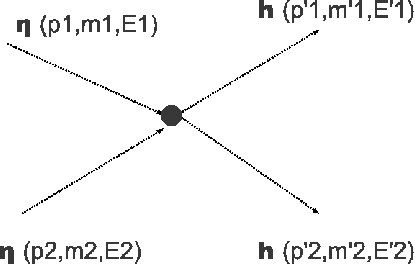
\includegraphics[width=0.5\textwidth]{1}%(eps preferiblemente)
    \caption[electrones]{Proceso donde dos etas se destruyen y se crean dos Higgs}
    \label{fi}
\end{figure*}
 



Por tanto el lagrangiano de interés es
\begin{equation}
L_{i}=\lambda_{l}h^{2}\eta_{0}^{2}
\label{4}
\end{equation}










\section{S-matriz}
 El orden a calcular la matriz $S$ es de orden uno ya que solo tenemos un termino de interacción \ref{4} el cual  determina el proceso de figuara \ref{fi}.\\
 Consideremos el proceso de la figura \ref{fi} donde $\eta(p_{1})\eta(p_{2})$ decae a un par de $h(p_{1}^{'})h(p_{2}^{'})$.
 El elemento de matriz $S_{fi}^{1}$ entre el estado inicial  y el estado final es 
 
 \begin{equation}
S_{fi}^{(1)}=-\lambda_{l}\int d^{4}x\bra{h(p_{1}^{'})h(p_{2}^{'})}h^{2}\eta_{0}^{2}\ket{\eta(p_{1})\eta(p_{2})}, 
 \label{5}
 \end{equation}
 
 sabemos que
 
 \begin{equation}
\eta_{0}=\eta_{+}+\eta_{-}=\frac{1}{\sqrt{2E_{p}V}}\left[ae^{-ip.x}+a^{+}e^{ip.x}\right]
 \label{6}
 \end{equation}

\begin{equation}
h=h_{+}+h_{-}=\frac{1}{\sqrt{2E_{p}V}}\left[ae^{-ip.x}+a^{+}e^{ip.x}\right]
 \label{7}
 \end{equation}


Por lo tanto
\begin{equation*}
h^{2}=\left(h_{+}+h_{-}\right)^{2}=(h_{+}+h_{-})(h_{+}+h_{-})
\end{equation*}
 \begin{equation}
=h_{+}h_{+}+h_{+}h_{-}+h_{-}h_{+}+h_{-}h_{-}
 \label{8}
 \end{equation}

\begin{equation*}
\eta_{0}^{2}=\left(\eta_{+}+\eta_{-}\right)^{2}=(\eta_{+}+\eta_{-})(\eta_{+}+\eta_{-})
\end{equation*}
\begin{equation}
=\eta_{+}\eta_{+}+\eta_{+}\eta_{-}+\eta_{-}\eta_{+}+\eta_{-}\eta_{-}
\label{9}
\end{equation}

El termino $\frac{1}{\sqrt{2E_{p}V}}$ de la expresión \ref{6} y \ref{7} es de normalización.\\

Calculemos  el termino $h^{2}\eta_{0}^{2}$:
\begin{equation*}
h^{2}\eta_{0}^{2}=(h_{+}h_{+}+h_{+}h_{-}+h_{-}h_{+}+h_{-}h_{-})(\eta_{+}\eta_{+}+\eta_{+}\eta_{-}+\eta_{-}\eta_{+}+\eta_{-}\eta_{-})
\end{equation*}
\begin{equation*}
=h_{+}h_{+}\eta_{+}\eta_{+}+h_{+}h_{+}\eta_{+}\eta_{-}+h_{+}h_{+}\eta_{-}\eta_{+}+h_{+}h_{+}\eta_{-}\eta_{-}+
\end{equation*}
\begin{equation*}
h_{+}h_{-}\eta_{+}\eta_{+}+h_{+}h_{-}\eta_{+}\eta_{-}+h_{+}h_{-}\eta_{-}\eta_{+}+h_{+}h_{-}\eta_{-}\eta_{-}+
\end{equation*}
\begin{equation*}
h_{-}h_{+}\eta_{+}\eta_{+}+h_{-}h_{+}\eta_{+}\eta_{-}+h_{-}h_{+}\eta_{-}\eta_{+}+h_{-}h_{+}\eta_{-}\eta_{-}+
\end{equation*}
\begin{equation}
h_{-}h_{-}\eta_{+}\eta_{+}+h_{-}h_{-}\eta_{+}\eta_{-}+h_{-}h_{-}\eta_{-}\eta_{+}+h_{-}h_{-}\eta_{-}\eta_{-}
\label{10}
\end{equation}
 Por otro lado  sabemos que 
 
 \begin{equation}
 h_{+}\ket{h}=\frac{1}{\sqrt{2E_{p}V}}e^{-ip.x}\ket0 ,\ h_{-}\ket{h}=\frac{1}{\sqrt{2E_{p}V}}e^{ip.x}\ket{1_{h}}
 \label{11}
 \end{equation}
 \begin{equation}
 \bra h h_{-}=\frac{1}{\sqrt{2E_{p}V}}e^{ip.x}\bra{0} ,\ \bra h h_{+}=\frac{1}{\sqrt{2E_{p}V}}e^{-ip.x}\bra{1_{h}}
 \label{12}
 \end{equation}


\begin{equation}
 \eta_{+}\ket{\eta}=\frac{1}{\sqrt{2E_{p}V}}e^{-ip.x}\ket0 ,\ \eta_{-}\ket{\eta}=\frac{1}{\sqrt{2E_{p}V}}e^{ip.x}\ket{1_{\eta}}
 \label{13}
 \end{equation}
 \begin{equation}
 \bra \eta \eta_{-}=\frac{1}{\sqrt{2E_{p}V}}e^{ip.x}\bra{0} ,\ \bra \eta \eta_{+}=\frac{1}{\sqrt{2E_{p}V}}e^{-ip.x}\bra {1_{\eta}}
 \label{14}
 \end{equation}
 
 y
 
 \begin{equation}
\bra{h(p_{1}^{'})h(p_{2}^{'})}h_{+}h_{+}=\frac{1}{\sqrt{2E_{p_{1}^{'}}V}}\frac{1}{\sqrt{2E_{p_{2}^{'}}V}}e^{-ip_{1}^{'}.x}e^{-ip_{2}^{'}.x}\bra{1_{h}1_{h}}
 \label{15}
 \end{equation}
\begin{equation}
\bra{h(p_{1}^{'})h(p_{2}^{'})}h_{+}h_{-}=\frac{1}{\sqrt{2E_{p_{1}^{'}}V}}\frac{1}{\sqrt{2E_{p_{2}^{'}}V}}e^{-ip_{1}^{'}.x}e^{ip_{2}^{'}.x}\bra{1_{h}0}
 \label{16}
 \end{equation}
\begin{equation}
\bra{h(p_{1}^{'})h(p_{2}^{'})}h_{-}h_{+}=\frac{1}{\sqrt{2E_{p_{1}^{'}}V}}\frac{1}{\sqrt{2E_{p_{2}^{'}}V}}e^{ip_{1}^{'}.x}e^{-ip_{2}^{'}.x}\bra{01_{h}}
 \label{17}
 \end{equation}
\begin{equation}
\bra{h(p_{1}^{'})h(p_{2}^{'})}h_{-}h_{-}=\frac{1}{\sqrt{2E_{p_{1}^{'}}V}}\frac{1}{\sqrt{2E_{p_{2}^{'}}V}}e^{ip_{1}^{'}.x}e^{ip_{2}^{'}.x}\bra{00}
 \label{18}
 \end{equation}

\begin{equation}
\eta_{+}\eta_{+}\ket{\eta(p_{1})\eta(p_{2})}=\frac{1}{\sqrt{2E_{p_{1}}V}}\frac{1}{\sqrt{2E_{p_{2}}V}}e^{-ip_{1}.x}e^{-ip_{2}.x}\ket{00}
 \label{19}
 \end{equation}


\begin{equation}
\eta_{+}\eta_{-}\ket{\eta(p_{1})\eta(p_{2})}=\frac{1}{\sqrt{2E_{p_{1}}V}}\frac{1}{\sqrt{2E_{p_{2}}V}}e^{-ip_{1}.x}e^{ip_{2}.x}\ket{01_{\eta}}
 \label{20}
 \end{equation}
\begin{equation}
\eta_{-}\eta_{+}\ket{\eta(p_{1})\eta(p_{2})}=\frac{1}{\sqrt{2E_{p_{1}}V}}\frac{1}{\sqrt{2E_{p_{2}}V}}e^{ip_{1}.x}e^{-ip_{2}.x}\ket{1_{\eta}0}
 \label{21}
 \end{equation}
\begin{equation}
\eta_{-}\eta_{-}\ket{\eta(p_{1})\eta(p_{2})}=\frac{1}{\sqrt{2E_{p_{1}}V}}\frac{1}{\sqrt{2E_{p_{2}}V}}e^{ip_{1}.x}e^{ip_{2}.x}\ket{1_{\eta}1_{\eta}}
 \label{22}
 \end{equation}

Por tanto san duchando el termino $h^{2}\eta_{0}^{2}$ con las relaciones desde \ref{15} hasta \ref{22} el termino que sobrevive es


\begin{equation*}
\bra{h(p_{1}^{'})h(p_{2}^{'})}h^{2}\eta_{0}^{2}\ket{\eta(p_{1})\eta(p_{2})}=\bra{h(p_{1}^{'})h(p_{2}^{'})}h_{-}h_{-}\eta_{+}\eta_{+}\ket{\eta(p_{1})\eta(p_{2})}
\end{equation*}
\begin{equation}
=\frac{1}{\sqrt{2E_{p_{1}^{'}}V}}\frac{1}{\sqrt{2E_{p_{2}^{'}}V}}\frac{1}{\sqrt{2E_{p_{1}}V}}\frac{1}{\sqrt{2E_{p_{2}}V}}e^{i(p_{1}^{'}+p_{2}^{'}-p_{1}-p_{2})}\bra{00}\ket{00}
\label{23}
\end{equation}

remplazando \ref{23} en matriz $S_{fi}^{(1)}$ obtenemos

\begin{equation}
S_{fi}^{(1)}=-i\lambda_{l}\frac{1}{\sqrt{2E_{p_{1}^{'}}V}}\frac{1}{\sqrt{2E_{p_{2}^{'}}V}}\frac{1}{\sqrt{2E_{p_{1}}V}}\frac{1}{\sqrt{2E_{p_{2}}V}}\int d^{4}x e^{i(p_{1}^{'}+p_{2}^{'}-p_{1}-p_{2})}\bra{00}\ket{00}
\label{24}
\end{equation}


El valor de la integral es $(2\pi)^{4}\delta^{4}(p_{1}+p_{2}-p_{1}^{'}-p_{2}^{'})$ y $\bra{00}\ket{00}=1$ por tanto el elemento de matriz obtenido es

\begin{equation}
S_{fi}^{(1)}=-i\lambda_{l}\frac{1}{\sqrt{2E_{p_{1}^{'}}V}}\frac{1}{\sqrt{2E_{p_{2}^{'}}V}}\frac{1}{\sqrt{2E_{p_{1}}V}}\frac{1}{\sqrt{2E_{p_{2}}V}}(2\pi)^{4}\delta^{4}(p_{1}+p_{2}-p_{1}^{'}-p_{2}^{'})
\label{25}
\end{equation}



\section{Process calculation}

 De la ecuación \ref{25} la función $\delta$  es la conservación de los $4$-momentos en el proceso general, el cual es multiplicado por $(2\pi)^{4}$. Hay un factor $(2EV)^{\frac{-1}{2} }$ para cada partícula del estado inicial y del estado final de energía $E$. El restos de termino de la expresión \ref{25} el cual depende sobre la naturaleza exacta de la interacción es llamada la amplitud de Feynman, es denotada por $iM_{fi}$.\\
 Para nuestro caso  
 \begin{equation}
iM_{fi}= -i\lambda_{l}
  \label{26}
 \end{equation}
              
   Para determinar la sección eficaz de nuestro modelo se determina a partir de expresión\cite{3}
   
   \begin{equation}
\frac{d\sigma}{d\Omega}=\frac{1}{64 \small{\pi} ^{2}s}\left[\frac{(s-(m_{1}^{'}+m_{2}^{'})^{2})(s-(m_{1}^{'}-m_{2}^{'})^{2}))}{(s-(m_{1}+m_{2})^{2})(s-(m_{1}-m_{2})^{2}))}\right]^{\frac{1}{2}}\overline{\vert M_{fi}\vert^{2}}
   \label{27}
   \end{equation}            
              
     Donde $m_{1}^{'}=m_{2}^{'}=m_{h}$ es la masa del Higgs, $m_{1}=m_{2}=m_{\eta}$ es la masa del eta y  $\overline{\vert M_{fi}\vert^{2}}=\lambda_{l}$ es la amplitud de Feynman, remplazando estos términos en la expresión \ref{27} se obtiene
     
     \begin{equation}
      \frac{d\sigma}{d\Omega}=\frac{1}{64\small{\pi} ^{2}s}\left[\frac{(s-4m_{h}^{2})}{(s-4m_{\eta}^{2})}\right]^{\frac{1}{2}}\left(\lambda_{l}\right)^{2}
          \label{28}
     \end{equation}
     
     
Con $s=\sqrt{E_{1}+E_{2}}$ y $E=\sqrt{p^{2}+m^{2}}$, la integral sobre $d\Omega$ es $4\pi$ por tanto la sección eficaz es 


\begin{equation}
  \sigma=\frac{(\lambda_{l})^{2}}{64\small{\pi} s}\left[\frac{(s-4m_{h}^{2})}{(s-4m_{\eta}^{2})}\right]^{\frac{1}{2}}
  \label{29}
\end{equation}  
          
     
     
Para determinar un valor númerico de la sección eficaz tomamos los siguientes valores: $ m_{\eta}=50GeV, m_{h}=120 GeV, \lambda_{l}=0.1$ y $\sqrt{s}=1016.68GeV $, Por tanto la expresión \ref{29} que así

\begin{equation*}
\sigma=\frac{(0.1)^{2}}{64\small{\pi} (1016.68GeV)^{2}}\left[\frac{(1016.68GeV)^{2}-4(120GeV)^{2}}{(1016.68GeV)^{2}-4(50GeV)^{2}}\right]^{\frac{1}{2}}
\label{30}GeV
\end{equation*}
     \begin{equation*}
    \frac{(0.1)^{2}}{64\small{\pi} (1016.68GeV)^{2}}\left[\frac{976055.3134 (GeV)^{2}}{1023638.232(GeV)^{2}}\right]^{\frac{1}{2}}
     \end{equation*}
              
\begin{equation*}
   = \frac{(0.1)^{2}}{64\small{\pi} (1016.68GeV)^{2}}(0,9764)
     \end{equation*}   
     \begin{equation}
    =4,69\times 10^{-11}(GeV)^{-2}
     \end{equation}              
              
\section{CalcHEP comparison}
Para ser la simulación se instala los programas de LanHep y CalHep.\\
Después se baja los archivos del proceso a simular de github, nuestro archivo pertinente es la carpeta idm para nuestro sistema. Se  instala la carpeta idm  en LanHep y CalHep y se ejecuta  CalHep desde el directorio idm para iniciar la simulación.\\
Los parámetros de la simulación son $~H0,~H0->H,H$ donde se descoge el diagrama de la figura \ref{fi} luego se ingresa los parámetros de la simulación que son $\lambda_{l}=0.1, m_{\eta}=50 GeV, m_{h}=120 GeV$, momento inicial $500 GeV$ y momento final es de $500GeV$ por tanto al sección eficaz de la simulación es de $0.145983[pb]$  

\section{Copyright}

\includegraphics[scale=0.5]{cc} Creative Commons Attribution-Share Alike 3.0 United States License.

\begin{thebibliography}{9}

\bibitem{1} D. Aristizabal Sierra, Jisuke Kubo and Daijiro Suematsu, Physical Review D 79, 013001 (2009)
\bibitem{2} Ernast Ma, Physical Review D 73, 0077301(2006)
\bibitem{3} Quantum Fiel Theory, Amitabha Lahiri and Palash B. Pal

\end{thebibliography}

%%% Local Variables: 
%%% mode: latex
%%% TeX-master: "qft_samples"
%%% End: 

% THDM I:  Yubian hep-ph/0504050
%
\chapter{$\eta \eta \to h h$}

Author:  Wady Alexander Ríos Herrera

Proceso: \textbf{Radiative seesaw II}\\

Experimentos de reactores  de neutrinos han demostrado que los neutrinos tienen masa.


\section{Lagrangian}


El modelo considerado es una extensión del modelo estándar, el contiene SU($2$)$\times$ U($1$)$_{Y}$ de singletes $N_{i}$ y un segundo doblete de Higgs $\eta$. En adición, una simetría discreta exacta $Z_{2}$ es asumida tal que el nuevo campo son impares bajo $Z_{2}$, mientras que en el modelo estándar son pares. El lagrangiano de interacción de  Yukawa inducido por el nuevo doblete Higgs es dada por  \cite{1}
\begin{equation}
L_{Y}=\epsilon _{ab}h_{\alpha j}\bar{N}_{j}P_{L}L_{\alpha}^{a}\eta ^{b}+H.c,
\label{1}
\end{equation}
 
L son doblete de leptón izquierdo, $\alpha , j$ son indices de generación (Greek indices etiquetado sabor leptonico e,$\mu$,$\tau$) y $\epsilon _{ab}$ es el tensor antisimetrico completo.\\

A partir del lagrangiano de interacción de Yukawa se determina el langrangiano interacción escalar cuadrático  \cite{2} 

\begin{equation}
L_{I}=\lambda_{3}(\Phi^{+}\Phi)( \eta^{+}\eta)+\lambda_{2}(\Phi^{+}\eta)( \eta^{+}\Phi) \frac{\lambda _{5}}{2}(\Phi^{+}\eta + H.C)
\label{2}
\end{equation}


Donde $\Phi$ es el modelo estándar del doblete de Higgs y es solo relevante para generación de masa neutrina. Ya que $Z_{2}$ es asumida  ser  exactamente simétrica del modelo $\eta$ tiene valor esperado del vacío cero. La Física escalar de los bosones son por lo tanto $R_{e}\Phi ^{0},\eta^{\pm},\eta_{0}^{R}\equiv Re\eta_{0}, \eta_{0}^{I}\equiv Im\eta_{0} =0 $ y $Im\eta^{+} =0$.\\


para ecuación \ref{2} se tiene que 
\begin{equation}
\Phi=\begin{pmatrix}
0 & \frac{h+v}{\sqrt{2}}
\end{pmatrix}, \ \eta= \begin{pmatrix}
\eta^{+} & \\
\eta_{0} & 
\end{pmatrix} 
\label{2.1}
\end{equation}

donde $h$ y $v$ son parámetros reales por tanto $\Phi =\Phi ^{+}$


Remplazando \ref{2.1} y las partes reales de $\eta$ el lagrangiano \ref{2} se determina el termina el termino relevante

\begin{equation*}
L_{I}=\lambda_{l} \left[\begin{pmatrix}
0 & \frac{h+v}{\sqrt{2}}
\end{pmatrix}\begin{pmatrix}
\eta^{+} & \\
\eta_{0} & 
\end{pmatrix}\right]^{2}= \lambda_{l}\left[0\eta^{+}+\left( \frac{h+v}{\sqrt{2}}\right)\eta_{0}\right]^{2}
\end{equation*}
\begin{equation*}
=\lambda_{l}(h+v)^{2}(\eta_{0})^{2}=\lambda_{l}(h^{2}+2hv+v^{2})(\eta_{0})^{2}
\end{equation*}
\begin{equation}
=\underbrace{\lambda_{l}h^{2}\eta_{0}^{2}}_{\star}+2\lambda_{l}hv\eta_{0}^{2}+\lambda_{l}v^{2}\eta_{0}^{2}, 
\label{3}
\end{equation}

Con 
\begin{equation}
\lambda_{l}=\frac{\lambda _{3}+\lambda _{4}+\lambda _{5}}{2}
\end{equation}

donde el termino relevante de la expresión \ref{3} es denotado con $\star$, ya que este genera el siguiente proceso 

\begin{figure*}[htb]
    \centering
    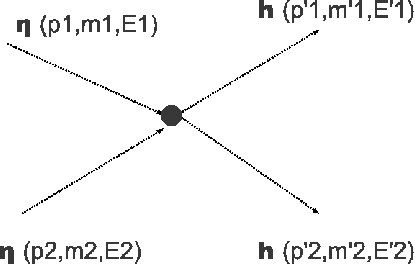
\includegraphics[width=0.5\textwidth]{1}%(eps preferiblemente)
    \caption[electrones]{Proceso donde dos etas se destruyen y se crean dos Higgs}
    \label{fi}
\end{figure*}
 



Por tanto el lagrangiano de interés es
\begin{equation}
L_{i}=\lambda_{l}h^{2}\eta_{0}^{2}
\label{4}
\end{equation}










\section{S-matriz}
 El orden a calcular la matriz $S$ es de orden uno ya que solo tenemos un termino de interacción \ref{4} el cual  determina el proceso de figuara \ref{fi}.\\
 Consideremos el proceso de la figura \ref{fi} donde $\eta(p_{1})\eta(p_{2})$ decae a un par de $h(p_{1}^{'})h(p_{2}^{'})$.
 El elemento de matriz $S_{fi}^{1}$ entre el estado inicial  y el estado final es 
 
 \begin{equation}
S_{fi}^{(1)}=-\lambda_{l}\int d^{4}x\bra{h(p_{1}^{'})h(p_{2}^{'})}h^{2}\eta_{0}^{2}\ket{\eta(p_{1})\eta(p_{2})}, 
 \label{5}
 \end{equation}
 
 sabemos que
 
 \begin{equation}
\eta_{0}=\eta_{+}+\eta_{-}=\frac{1}{\sqrt{2E_{p}V}}\left[ae^{-ip.x}+a^{+}e^{ip.x}\right]
 \label{6}
 \end{equation}

\begin{equation}
h=h_{+}+h_{-}=\frac{1}{\sqrt{2E_{p}V}}\left[ae^{-ip.x}+a^{+}e^{ip.x}\right]
 \label{7}
 \end{equation}


Por lo tanto
\begin{equation*}
h^{2}=\left(h_{+}+h_{-}\right)^{2}=(h_{+}+h_{-})(h_{+}+h_{-})
\end{equation*}
 \begin{equation}
=h_{+}h_{+}+h_{+}h_{-}+h_{-}h_{+}+h_{-}h_{-}
 \label{8}
 \end{equation}

\begin{equation*}
\eta_{0}^{2}=\left(\eta_{+}+\eta_{-}\right)^{2}=(\eta_{+}+\eta_{-})(\eta_{+}+\eta_{-})
\end{equation*}
\begin{equation}
=\eta_{+}\eta_{+}+\eta_{+}\eta_{-}+\eta_{-}\eta_{+}+\eta_{-}\eta_{-}
\label{9}
\end{equation}

El termino $\frac{1}{\sqrt{2E_{p}V}}$ de la expresión \ref{6} y \ref{7} es de normalización.\\

Calculemos  el termino $h^{2}\eta_{0}^{2}$:
\begin{equation*}
h^{2}\eta_{0}^{2}=(h_{+}h_{+}+h_{+}h_{-}+h_{-}h_{+}+h_{-}h_{-})(\eta_{+}\eta_{+}+\eta_{+}\eta_{-}+\eta_{-}\eta_{+}+\eta_{-}\eta_{-})
\end{equation*}
\begin{equation*}
=h_{+}h_{+}\eta_{+}\eta_{+}+h_{+}h_{+}\eta_{+}\eta_{-}+h_{+}h_{+}\eta_{-}\eta_{+}+h_{+}h_{+}\eta_{-}\eta_{-}+
\end{equation*}
\begin{equation*}
h_{+}h_{-}\eta_{+}\eta_{+}+h_{+}h_{-}\eta_{+}\eta_{-}+h_{+}h_{-}\eta_{-}\eta_{+}+h_{+}h_{-}\eta_{-}\eta_{-}+
\end{equation*}
\begin{equation*}
h_{-}h_{+}\eta_{+}\eta_{+}+h_{-}h_{+}\eta_{+}\eta_{-}+h_{-}h_{+}\eta_{-}\eta_{+}+h_{-}h_{+}\eta_{-}\eta_{-}+
\end{equation*}
\begin{equation}
h_{-}h_{-}\eta_{+}\eta_{+}+h_{-}h_{-}\eta_{+}\eta_{-}+h_{-}h_{-}\eta_{-}\eta_{+}+h_{-}h_{-}\eta_{-}\eta_{-}
\label{10}
\end{equation}
 Por otro lado  sabemos que 
 
 \begin{equation}
 h_{+}\ket{h}=\frac{1}{\sqrt{2E_{p}V}}e^{-ip.x}\ket0 ,\ h_{-}\ket{h}=\frac{1}{\sqrt{2E_{p}V}}e^{ip.x}\ket{1_{h}}
 \label{11}
 \end{equation}
 \begin{equation}
 \bra h h_{-}=\frac{1}{\sqrt{2E_{p}V}}e^{ip.x}\bra{0} ,\ \bra h h_{+}=\frac{1}{\sqrt{2E_{p}V}}e^{-ip.x}\bra{1_{h}}
 \label{12}
 \end{equation}


\begin{equation}
 \eta_{+}\ket{\eta}=\frac{1}{\sqrt{2E_{p}V}}e^{-ip.x}\ket0 ,\ \eta_{-}\ket{\eta}=\frac{1}{\sqrt{2E_{p}V}}e^{ip.x}\ket{1_{\eta}}
 \label{13}
 \end{equation}
 \begin{equation}
 \bra \eta \eta_{-}=\frac{1}{\sqrt{2E_{p}V}}e^{ip.x}\bra{0} ,\ \bra \eta \eta_{+}=\frac{1}{\sqrt{2E_{p}V}}e^{-ip.x}\bra {1_{\eta}}
 \label{14}
 \end{equation}
 
 y
 
 \begin{equation}
\bra{h(p_{1}^{'})h(p_{2}^{'})}h_{+}h_{+}=\frac{1}{\sqrt{2E_{p_{1}^{'}}V}}\frac{1}{\sqrt{2E_{p_{2}^{'}}V}}e^{-ip_{1}^{'}.x}e^{-ip_{2}^{'}.x}\bra{1_{h}1_{h}}
 \label{15}
 \end{equation}
\begin{equation}
\bra{h(p_{1}^{'})h(p_{2}^{'})}h_{+}h_{-}=\frac{1}{\sqrt{2E_{p_{1}^{'}}V}}\frac{1}{\sqrt{2E_{p_{2}^{'}}V}}e^{-ip_{1}^{'}.x}e^{ip_{2}^{'}.x}\bra{1_{h}0}
 \label{16}
 \end{equation}
\begin{equation}
\bra{h(p_{1}^{'})h(p_{2}^{'})}h_{-}h_{+}=\frac{1}{\sqrt{2E_{p_{1}^{'}}V}}\frac{1}{\sqrt{2E_{p_{2}^{'}}V}}e^{ip_{1}^{'}.x}e^{-ip_{2}^{'}.x}\bra{01_{h}}
 \label{17}
 \end{equation}
\begin{equation}
\bra{h(p_{1}^{'})h(p_{2}^{'})}h_{-}h_{-}=\frac{1}{\sqrt{2E_{p_{1}^{'}}V}}\frac{1}{\sqrt{2E_{p_{2}^{'}}V}}e^{ip_{1}^{'}.x}e^{ip_{2}^{'}.x}\bra{00}
 \label{18}
 \end{equation}

\begin{equation}
\eta_{+}\eta_{+}\ket{\eta(p_{1})\eta(p_{2})}=\frac{1}{\sqrt{2E_{p_{1}}V}}\frac{1}{\sqrt{2E_{p_{2}}V}}e^{-ip_{1}.x}e^{-ip_{2}.x}\ket{00}
 \label{19}
 \end{equation}


\begin{equation}
\eta_{+}\eta_{-}\ket{\eta(p_{1})\eta(p_{2})}=\frac{1}{\sqrt{2E_{p_{1}}V}}\frac{1}{\sqrt{2E_{p_{2}}V}}e^{-ip_{1}.x}e^{ip_{2}.x}\ket{01_{\eta}}
 \label{20}
 \end{equation}
\begin{equation}
\eta_{-}\eta_{+}\ket{\eta(p_{1})\eta(p_{2})}=\frac{1}{\sqrt{2E_{p_{1}}V}}\frac{1}{\sqrt{2E_{p_{2}}V}}e^{ip_{1}.x}e^{-ip_{2}.x}\ket{1_{\eta}0}
 \label{21}
 \end{equation}
\begin{equation}
\eta_{-}\eta_{-}\ket{\eta(p_{1})\eta(p_{2})}=\frac{1}{\sqrt{2E_{p_{1}}V}}\frac{1}{\sqrt{2E_{p_{2}}V}}e^{ip_{1}.x}e^{ip_{2}.x}\ket{1_{\eta}1_{\eta}}
 \label{22}
 \end{equation}

Por tanto san duchando el termino $h^{2}\eta_{0}^{2}$ con las relaciones desde \ref{15} hasta \ref{22} el termino que sobrevive es


\begin{equation*}
\bra{h(p_{1}^{'})h(p_{2}^{'})}h^{2}\eta_{0}^{2}\ket{\eta(p_{1})\eta(p_{2})}=\bra{h(p_{1}^{'})h(p_{2}^{'})}h_{-}h_{-}\eta_{+}\eta_{+}\ket{\eta(p_{1})\eta(p_{2})}
\end{equation*}
\begin{equation}
=\frac{1}{\sqrt{2E_{p_{1}^{'}}V}}\frac{1}{\sqrt{2E_{p_{2}^{'}}V}}\frac{1}{\sqrt{2E_{p_{1}}V}}\frac{1}{\sqrt{2E_{p_{2}}V}}e^{i(p_{1}^{'}+p_{2}^{'}-p_{1}-p_{2})}\bra{00}\ket{00}
\label{23}
\end{equation}

remplazando \ref{23} en matriz $S_{fi}^{(1)}$ obtenemos

\begin{equation}
S_{fi}^{(1)}=-i\lambda_{l}\frac{1}{\sqrt{2E_{p_{1}^{'}}V}}\frac{1}{\sqrt{2E_{p_{2}^{'}}V}}\frac{1}{\sqrt{2E_{p_{1}}V}}\frac{1}{\sqrt{2E_{p_{2}}V}}\int d^{4}x e^{i(p_{1}^{'}+p_{2}^{'}-p_{1}-p_{2})}\bra{00}\ket{00}
\label{24}
\end{equation}


El valor de la integral es $(2\pi)^{4}\delta^{4}(p_{1}+p_{2}-p_{1}^{'}-p_{2}^{'})$ y $\bra{00}\ket{00}=1$ por tanto el elemento de matriz obtenido es

\begin{equation}
S_{fi}^{(1)}=-i\lambda_{l}\frac{1}{\sqrt{2E_{p_{1}^{'}}V}}\frac{1}{\sqrt{2E_{p_{2}^{'}}V}}\frac{1}{\sqrt{2E_{p_{1}}V}}\frac{1}{\sqrt{2E_{p_{2}}V}}(2\pi)^{4}\delta^{4}(p_{1}+p_{2}-p_{1}^{'}-p_{2}^{'})
\label{25}
\end{equation}



\section{Process calculation}

 De la ecuación \ref{25} la función $\delta$  es la conservación de los $4$-momentos en el proceso general, el cual es multiplicado por $(2\pi)^{4}$. Hay un factor $(2EV)^{\frac{-1}{2} }$ para cada partícula del estado inicial y del estado final de energía $E$. El restos de termino de la expresión \ref{25} el cual depende sobre la naturaleza exacta de la interacción es llamada la amplitud de Feynman, es denotada por $iM_{fi}$.\\
 Para nuestro caso  
 \begin{equation}
iM_{fi}= -i\lambda_{l}
  \label{26}
 \end{equation}
              
   Para determinar la sección eficaz de nuestro modelo se determina a partir de expresión\cite{3}
   
   \begin{equation}
\frac{d\sigma}{d\Omega}=\frac{1}{64 \small{\pi} ^{2}s}\left[\frac{(s-(m_{1}^{'}+m_{2}^{'})^{2})(s-(m_{1}^{'}-m_{2}^{'})^{2}))}{(s-(m_{1}+m_{2})^{2})(s-(m_{1}-m_{2})^{2}))}\right]^{\frac{1}{2}}\overline{\vert M_{fi}\vert^{2}}
   \label{27}
   \end{equation}            
              
     Donde $m_{1}^{'}=m_{2}^{'}=m_{h}$ es la masa del Higgs, $m_{1}=m_{2}=m_{\eta}$ es la masa del eta y  $\overline{\vert M_{fi}\vert^{2}}=\lambda_{l}$ es la amplitud de Feynman, remplazando estos términos en la expresión \ref{27} se obtiene
     
     \begin{equation}
      \frac{d\sigma}{d\Omega}=\frac{1}{64\small{\pi} ^{2}s}\left[\frac{(s-4m_{h}^{2})}{(s-4m_{\eta}^{2})}\right]^{\frac{1}{2}}\left(\lambda_{l}\right)^{2}
          \label{28}
     \end{equation}
     
     
Con $s=\sqrt{E_{1}+E_{2}}$ y $E=\sqrt{p^{2}+m^{2}}$, la integral sobre $d\Omega$ es $4\pi$ por tanto la sección eficaz es 


\begin{equation}
  \sigma=\frac{(\lambda_{l})^{2}}{64\small{\pi} s}\left[\frac{(s-4m_{h}^{2})}{(s-4m_{\eta}^{2})}\right]^{\frac{1}{2}}
  \label{29}
\end{equation}  
          
     
     
Para determinar un valor númerico de la sección eficaz tomamos los siguientes valores: $ m_{\eta}=50GeV, m_{h}=120 GeV, \lambda_{l}=0.1$ y $\sqrt{s}=1016.68GeV $, Por tanto la expresión \ref{29} que así

\begin{equation*}
\sigma=\frac{(0.1)^{2}}{64\small{\pi} (1016.68GeV)^{2}}\left[\frac{(1016.68GeV)^{2}-4(120GeV)^{2}}{(1016.68GeV)^{2}-4(50GeV)^{2}}\right]^{\frac{1}{2}}
\label{30}GeV
\end{equation*}
     \begin{equation*}
    \frac{(0.1)^{2}}{64\small{\pi} (1016.68GeV)^{2}}\left[\frac{976055.3134 (GeV)^{2}}{1023638.232(GeV)^{2}}\right]^{\frac{1}{2}}
     \end{equation*}
              
\begin{equation*}
   = \frac{(0.1)^{2}}{64\small{\pi} (1016.68GeV)^{2}}(0,9764)
     \end{equation*}   
     \begin{equation}
    =4,69\times 10^{-11}(GeV)^{-2}
     \end{equation}              
              
\section{CalcHEP comparison}
Para ser la simulación se instala los programas de LanHep y CalHep.\\
Después se baja los archivos del proceso a simular de github, nuestro archivo pertinente es la carpeta idm para nuestro sistema. Se  instala la carpeta idm  en LanHep y CalHep y se ejecuta  CalHep desde el directorio idm para iniciar la simulación.\\
Los parámetros de la simulación son $~H0,~H0->H,H$ donde se descoge el diagrama de la figura \ref{fi} luego se ingresa los parámetros de la simulación que son $\lambda_{l}=0.1, m_{\eta}=50 GeV, m_{h}=120 GeV$, momento inicial $500 GeV$ y momento final es de $500GeV$ por tanto al sección eficaz de la simulación es de $0.145983[pb]$  

\section{Copyright}

\includegraphics[scale=0.5]{cc} Creative Commons Attribution-Share Alike 3.0 United States License.

\begin{thebibliography}{9}

\bibitem{1} D. Aristizabal Sierra, Jisuke Kubo and Daijiro Suematsu, Physical Review D 79, 013001 (2009)
\bibitem{2} Ernast Ma, Physical Review D 73, 0077301(2006)
\bibitem{3} Quantum Fiel Theory, Amitabha Lahiri and Palash B. Pal

\end{thebibliography}

%%% Local Variables: 
%%% mode: latex
%%% TeX-master: "qft_samples"
%%% End: 

% THDM II: Oscar Andrés hep-ph/0504050
%
\chapter{$\eta \eta \to h h$}

Author:  Wady Alexander Ríos Herrera

Proceso: \textbf{Radiative seesaw II}\\

Experimentos de reactores  de neutrinos han demostrado que los neutrinos tienen masa.


\section{Lagrangian}


El modelo considerado es una extensión del modelo estándar, el contiene SU($2$)$\times$ U($1$)$_{Y}$ de singletes $N_{i}$ y un segundo doblete de Higgs $\eta$. En adición, una simetría discreta exacta $Z_{2}$ es asumida tal que el nuevo campo son impares bajo $Z_{2}$, mientras que en el modelo estándar son pares. El lagrangiano de interacción de  Yukawa inducido por el nuevo doblete Higgs es dada por  \cite{1}
\begin{equation}
L_{Y}=\epsilon _{ab}h_{\alpha j}\bar{N}_{j}P_{L}L_{\alpha}^{a}\eta ^{b}+H.c,
\label{1}
\end{equation}
 
L son doblete de leptón izquierdo, $\alpha , j$ son indices de generación (Greek indices etiquetado sabor leptonico e,$\mu$,$\tau$) y $\epsilon _{ab}$ es el tensor antisimetrico completo.\\

A partir del lagrangiano de interacción de Yukawa se determina el langrangiano interacción escalar cuadrático  \cite{2} 

\begin{equation}
L_{I}=\lambda_{3}(\Phi^{+}\Phi)( \eta^{+}\eta)+\lambda_{2}(\Phi^{+}\eta)( \eta^{+}\Phi) \frac{\lambda _{5}}{2}(\Phi^{+}\eta + H.C)
\label{2}
\end{equation}


Donde $\Phi$ es el modelo estándar del doblete de Higgs y es solo relevante para generación de masa neutrina. Ya que $Z_{2}$ es asumida  ser  exactamente simétrica del modelo $\eta$ tiene valor esperado del vacío cero. La Física escalar de los bosones son por lo tanto $R_{e}\Phi ^{0},\eta^{\pm},\eta_{0}^{R}\equiv Re\eta_{0}, \eta_{0}^{I}\equiv Im\eta_{0} =0 $ y $Im\eta^{+} =0$.\\


para ecuación \ref{2} se tiene que 
\begin{equation}
\Phi=\begin{pmatrix}
0 & \frac{h+v}{\sqrt{2}}
\end{pmatrix}, \ \eta= \begin{pmatrix}
\eta^{+} & \\
\eta_{0} & 
\end{pmatrix} 
\label{2.1}
\end{equation}

donde $h$ y $v$ son parámetros reales por tanto $\Phi =\Phi ^{+}$


Remplazando \ref{2.1} y las partes reales de $\eta$ el lagrangiano \ref{2} se determina el termina el termino relevante

\begin{equation*}
L_{I}=\lambda_{l} \left[\begin{pmatrix}
0 & \frac{h+v}{\sqrt{2}}
\end{pmatrix}\begin{pmatrix}
\eta^{+} & \\
\eta_{0} & 
\end{pmatrix}\right]^{2}= \lambda_{l}\left[0\eta^{+}+\left( \frac{h+v}{\sqrt{2}}\right)\eta_{0}\right]^{2}
\end{equation*}
\begin{equation*}
=\lambda_{l}(h+v)^{2}(\eta_{0})^{2}=\lambda_{l}(h^{2}+2hv+v^{2})(\eta_{0})^{2}
\end{equation*}
\begin{equation}
=\underbrace{\lambda_{l}h^{2}\eta_{0}^{2}}_{\star}+2\lambda_{l}hv\eta_{0}^{2}+\lambda_{l}v^{2}\eta_{0}^{2}, 
\label{3}
\end{equation}

Con 
\begin{equation}
\lambda_{l}=\frac{\lambda _{3}+\lambda _{4}+\lambda _{5}}{2}
\end{equation}

donde el termino relevante de la expresión \ref{3} es denotado con $\star$, ya que este genera el siguiente proceso 

\begin{figure*}[htb]
    \centering
    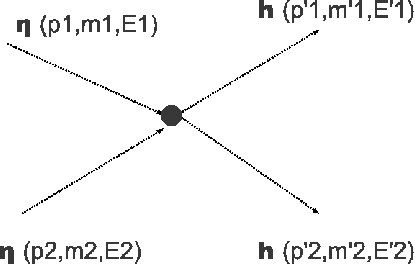
\includegraphics[width=0.5\textwidth]{1}%(eps preferiblemente)
    \caption[electrones]{Proceso donde dos etas se destruyen y se crean dos Higgs}
    \label{fi}
\end{figure*}
 



Por tanto el lagrangiano de interés es
\begin{equation}
L_{i}=\lambda_{l}h^{2}\eta_{0}^{2}
\label{4}
\end{equation}










\section{S-matriz}
 El orden a calcular la matriz $S$ es de orden uno ya que solo tenemos un termino de interacción \ref{4} el cual  determina el proceso de figuara \ref{fi}.\\
 Consideremos el proceso de la figura \ref{fi} donde $\eta(p_{1})\eta(p_{2})$ decae a un par de $h(p_{1}^{'})h(p_{2}^{'})$.
 El elemento de matriz $S_{fi}^{1}$ entre el estado inicial  y el estado final es 
 
 \begin{equation}
S_{fi}^{(1)}=-\lambda_{l}\int d^{4}x\bra{h(p_{1}^{'})h(p_{2}^{'})}h^{2}\eta_{0}^{2}\ket{\eta(p_{1})\eta(p_{2})}, 
 \label{5}
 \end{equation}
 
 sabemos que
 
 \begin{equation}
\eta_{0}=\eta_{+}+\eta_{-}=\frac{1}{\sqrt{2E_{p}V}}\left[ae^{-ip.x}+a^{+}e^{ip.x}\right]
 \label{6}
 \end{equation}

\begin{equation}
h=h_{+}+h_{-}=\frac{1}{\sqrt{2E_{p}V}}\left[ae^{-ip.x}+a^{+}e^{ip.x}\right]
 \label{7}
 \end{equation}


Por lo tanto
\begin{equation*}
h^{2}=\left(h_{+}+h_{-}\right)^{2}=(h_{+}+h_{-})(h_{+}+h_{-})
\end{equation*}
 \begin{equation}
=h_{+}h_{+}+h_{+}h_{-}+h_{-}h_{+}+h_{-}h_{-}
 \label{8}
 \end{equation}

\begin{equation*}
\eta_{0}^{2}=\left(\eta_{+}+\eta_{-}\right)^{2}=(\eta_{+}+\eta_{-})(\eta_{+}+\eta_{-})
\end{equation*}
\begin{equation}
=\eta_{+}\eta_{+}+\eta_{+}\eta_{-}+\eta_{-}\eta_{+}+\eta_{-}\eta_{-}
\label{9}
\end{equation}

El termino $\frac{1}{\sqrt{2E_{p}V}}$ de la expresión \ref{6} y \ref{7} es de normalización.\\

Calculemos  el termino $h^{2}\eta_{0}^{2}$:
\begin{equation*}
h^{2}\eta_{0}^{2}=(h_{+}h_{+}+h_{+}h_{-}+h_{-}h_{+}+h_{-}h_{-})(\eta_{+}\eta_{+}+\eta_{+}\eta_{-}+\eta_{-}\eta_{+}+\eta_{-}\eta_{-})
\end{equation*}
\begin{equation*}
=h_{+}h_{+}\eta_{+}\eta_{+}+h_{+}h_{+}\eta_{+}\eta_{-}+h_{+}h_{+}\eta_{-}\eta_{+}+h_{+}h_{+}\eta_{-}\eta_{-}+
\end{equation*}
\begin{equation*}
h_{+}h_{-}\eta_{+}\eta_{+}+h_{+}h_{-}\eta_{+}\eta_{-}+h_{+}h_{-}\eta_{-}\eta_{+}+h_{+}h_{-}\eta_{-}\eta_{-}+
\end{equation*}
\begin{equation*}
h_{-}h_{+}\eta_{+}\eta_{+}+h_{-}h_{+}\eta_{+}\eta_{-}+h_{-}h_{+}\eta_{-}\eta_{+}+h_{-}h_{+}\eta_{-}\eta_{-}+
\end{equation*}
\begin{equation}
h_{-}h_{-}\eta_{+}\eta_{+}+h_{-}h_{-}\eta_{+}\eta_{-}+h_{-}h_{-}\eta_{-}\eta_{+}+h_{-}h_{-}\eta_{-}\eta_{-}
\label{10}
\end{equation}
 Por otro lado  sabemos que 
 
 \begin{equation}
 h_{+}\ket{h}=\frac{1}{\sqrt{2E_{p}V}}e^{-ip.x}\ket0 ,\ h_{-}\ket{h}=\frac{1}{\sqrt{2E_{p}V}}e^{ip.x}\ket{1_{h}}
 \label{11}
 \end{equation}
 \begin{equation}
 \bra h h_{-}=\frac{1}{\sqrt{2E_{p}V}}e^{ip.x}\bra{0} ,\ \bra h h_{+}=\frac{1}{\sqrt{2E_{p}V}}e^{-ip.x}\bra{1_{h}}
 \label{12}
 \end{equation}


\begin{equation}
 \eta_{+}\ket{\eta}=\frac{1}{\sqrt{2E_{p}V}}e^{-ip.x}\ket0 ,\ \eta_{-}\ket{\eta}=\frac{1}{\sqrt{2E_{p}V}}e^{ip.x}\ket{1_{\eta}}
 \label{13}
 \end{equation}
 \begin{equation}
 \bra \eta \eta_{-}=\frac{1}{\sqrt{2E_{p}V}}e^{ip.x}\bra{0} ,\ \bra \eta \eta_{+}=\frac{1}{\sqrt{2E_{p}V}}e^{-ip.x}\bra {1_{\eta}}
 \label{14}
 \end{equation}
 
 y
 
 \begin{equation}
\bra{h(p_{1}^{'})h(p_{2}^{'})}h_{+}h_{+}=\frac{1}{\sqrt{2E_{p_{1}^{'}}V}}\frac{1}{\sqrt{2E_{p_{2}^{'}}V}}e^{-ip_{1}^{'}.x}e^{-ip_{2}^{'}.x}\bra{1_{h}1_{h}}
 \label{15}
 \end{equation}
\begin{equation}
\bra{h(p_{1}^{'})h(p_{2}^{'})}h_{+}h_{-}=\frac{1}{\sqrt{2E_{p_{1}^{'}}V}}\frac{1}{\sqrt{2E_{p_{2}^{'}}V}}e^{-ip_{1}^{'}.x}e^{ip_{2}^{'}.x}\bra{1_{h}0}
 \label{16}
 \end{equation}
\begin{equation}
\bra{h(p_{1}^{'})h(p_{2}^{'})}h_{-}h_{+}=\frac{1}{\sqrt{2E_{p_{1}^{'}}V}}\frac{1}{\sqrt{2E_{p_{2}^{'}}V}}e^{ip_{1}^{'}.x}e^{-ip_{2}^{'}.x}\bra{01_{h}}
 \label{17}
 \end{equation}
\begin{equation}
\bra{h(p_{1}^{'})h(p_{2}^{'})}h_{-}h_{-}=\frac{1}{\sqrt{2E_{p_{1}^{'}}V}}\frac{1}{\sqrt{2E_{p_{2}^{'}}V}}e^{ip_{1}^{'}.x}e^{ip_{2}^{'}.x}\bra{00}
 \label{18}
 \end{equation}

\begin{equation}
\eta_{+}\eta_{+}\ket{\eta(p_{1})\eta(p_{2})}=\frac{1}{\sqrt{2E_{p_{1}}V}}\frac{1}{\sqrt{2E_{p_{2}}V}}e^{-ip_{1}.x}e^{-ip_{2}.x}\ket{00}
 \label{19}
 \end{equation}


\begin{equation}
\eta_{+}\eta_{-}\ket{\eta(p_{1})\eta(p_{2})}=\frac{1}{\sqrt{2E_{p_{1}}V}}\frac{1}{\sqrt{2E_{p_{2}}V}}e^{-ip_{1}.x}e^{ip_{2}.x}\ket{01_{\eta}}
 \label{20}
 \end{equation}
\begin{equation}
\eta_{-}\eta_{+}\ket{\eta(p_{1})\eta(p_{2})}=\frac{1}{\sqrt{2E_{p_{1}}V}}\frac{1}{\sqrt{2E_{p_{2}}V}}e^{ip_{1}.x}e^{-ip_{2}.x}\ket{1_{\eta}0}
 \label{21}
 \end{equation}
\begin{equation}
\eta_{-}\eta_{-}\ket{\eta(p_{1})\eta(p_{2})}=\frac{1}{\sqrt{2E_{p_{1}}V}}\frac{1}{\sqrt{2E_{p_{2}}V}}e^{ip_{1}.x}e^{ip_{2}.x}\ket{1_{\eta}1_{\eta}}
 \label{22}
 \end{equation}

Por tanto san duchando el termino $h^{2}\eta_{0}^{2}$ con las relaciones desde \ref{15} hasta \ref{22} el termino que sobrevive es


\begin{equation*}
\bra{h(p_{1}^{'})h(p_{2}^{'})}h^{2}\eta_{0}^{2}\ket{\eta(p_{1})\eta(p_{2})}=\bra{h(p_{1}^{'})h(p_{2}^{'})}h_{-}h_{-}\eta_{+}\eta_{+}\ket{\eta(p_{1})\eta(p_{2})}
\end{equation*}
\begin{equation}
=\frac{1}{\sqrt{2E_{p_{1}^{'}}V}}\frac{1}{\sqrt{2E_{p_{2}^{'}}V}}\frac{1}{\sqrt{2E_{p_{1}}V}}\frac{1}{\sqrt{2E_{p_{2}}V}}e^{i(p_{1}^{'}+p_{2}^{'}-p_{1}-p_{2})}\bra{00}\ket{00}
\label{23}
\end{equation}

remplazando \ref{23} en matriz $S_{fi}^{(1)}$ obtenemos

\begin{equation}
S_{fi}^{(1)}=-i\lambda_{l}\frac{1}{\sqrt{2E_{p_{1}^{'}}V}}\frac{1}{\sqrt{2E_{p_{2}^{'}}V}}\frac{1}{\sqrt{2E_{p_{1}}V}}\frac{1}{\sqrt{2E_{p_{2}}V}}\int d^{4}x e^{i(p_{1}^{'}+p_{2}^{'}-p_{1}-p_{2})}\bra{00}\ket{00}
\label{24}
\end{equation}


El valor de la integral es $(2\pi)^{4}\delta^{4}(p_{1}+p_{2}-p_{1}^{'}-p_{2}^{'})$ y $\bra{00}\ket{00}=1$ por tanto el elemento de matriz obtenido es

\begin{equation}
S_{fi}^{(1)}=-i\lambda_{l}\frac{1}{\sqrt{2E_{p_{1}^{'}}V}}\frac{1}{\sqrt{2E_{p_{2}^{'}}V}}\frac{1}{\sqrt{2E_{p_{1}}V}}\frac{1}{\sqrt{2E_{p_{2}}V}}(2\pi)^{4}\delta^{4}(p_{1}+p_{2}-p_{1}^{'}-p_{2}^{'})
\label{25}
\end{equation}



\section{Process calculation}

 De la ecuación \ref{25} la función $\delta$  es la conservación de los $4$-momentos en el proceso general, el cual es multiplicado por $(2\pi)^{4}$. Hay un factor $(2EV)^{\frac{-1}{2} }$ para cada partícula del estado inicial y del estado final de energía $E$. El restos de termino de la expresión \ref{25} el cual depende sobre la naturaleza exacta de la interacción es llamada la amplitud de Feynman, es denotada por $iM_{fi}$.\\
 Para nuestro caso  
 \begin{equation}
iM_{fi}= -i\lambda_{l}
  \label{26}
 \end{equation}
              
   Para determinar la sección eficaz de nuestro modelo se determina a partir de expresión\cite{3}
   
   \begin{equation}
\frac{d\sigma}{d\Omega}=\frac{1}{64 \small{\pi} ^{2}s}\left[\frac{(s-(m_{1}^{'}+m_{2}^{'})^{2})(s-(m_{1}^{'}-m_{2}^{'})^{2}))}{(s-(m_{1}+m_{2})^{2})(s-(m_{1}-m_{2})^{2}))}\right]^{\frac{1}{2}}\overline{\vert M_{fi}\vert^{2}}
   \label{27}
   \end{equation}            
              
     Donde $m_{1}^{'}=m_{2}^{'}=m_{h}$ es la masa del Higgs, $m_{1}=m_{2}=m_{\eta}$ es la masa del eta y  $\overline{\vert M_{fi}\vert^{2}}=\lambda_{l}$ es la amplitud de Feynman, remplazando estos términos en la expresión \ref{27} se obtiene
     
     \begin{equation}
      \frac{d\sigma}{d\Omega}=\frac{1}{64\small{\pi} ^{2}s}\left[\frac{(s-4m_{h}^{2})}{(s-4m_{\eta}^{2})}\right]^{\frac{1}{2}}\left(\lambda_{l}\right)^{2}
          \label{28}
     \end{equation}
     
     
Con $s=\sqrt{E_{1}+E_{2}}$ y $E=\sqrt{p^{2}+m^{2}}$, la integral sobre $d\Omega$ es $4\pi$ por tanto la sección eficaz es 


\begin{equation}
  \sigma=\frac{(\lambda_{l})^{2}}{64\small{\pi} s}\left[\frac{(s-4m_{h}^{2})}{(s-4m_{\eta}^{2})}\right]^{\frac{1}{2}}
  \label{29}
\end{equation}  
          
     
     
Para determinar un valor númerico de la sección eficaz tomamos los siguientes valores: $ m_{\eta}=50GeV, m_{h}=120 GeV, \lambda_{l}=0.1$ y $\sqrt{s}=1016.68GeV $, Por tanto la expresión \ref{29} que así

\begin{equation*}
\sigma=\frac{(0.1)^{2}}{64\small{\pi} (1016.68GeV)^{2}}\left[\frac{(1016.68GeV)^{2}-4(120GeV)^{2}}{(1016.68GeV)^{2}-4(50GeV)^{2}}\right]^{\frac{1}{2}}
\label{30}GeV
\end{equation*}
     \begin{equation*}
    \frac{(0.1)^{2}}{64\small{\pi} (1016.68GeV)^{2}}\left[\frac{976055.3134 (GeV)^{2}}{1023638.232(GeV)^{2}}\right]^{\frac{1}{2}}
     \end{equation*}
              
\begin{equation*}
   = \frac{(0.1)^{2}}{64\small{\pi} (1016.68GeV)^{2}}(0,9764)
     \end{equation*}   
     \begin{equation}
    =4,69\times 10^{-11}(GeV)^{-2}
     \end{equation}              
              
\section{CalcHEP comparison}
Para ser la simulación se instala los programas de LanHep y CalHep.\\
Después se baja los archivos del proceso a simular de github, nuestro archivo pertinente es la carpeta idm para nuestro sistema. Se  instala la carpeta idm  en LanHep y CalHep y se ejecuta  CalHep desde el directorio idm para iniciar la simulación.\\
Los parámetros de la simulación son $~H0,~H0->H,H$ donde se descoge el diagrama de la figura \ref{fi} luego se ingresa los parámetros de la simulación que son $\lambda_{l}=0.1, m_{\eta}=50 GeV, m_{h}=120 GeV$, momento inicial $500 GeV$ y momento final es de $500GeV$ por tanto al sección eficaz de la simulación es de $0.145983[pb]$  

\section{Copyright}

\includegraphics[scale=0.5]{cc} Creative Commons Attribution-Share Alike 3.0 United States License.

\begin{thebibliography}{9}

\bibitem{1} D. Aristizabal Sierra, Jisuke Kubo and Daijiro Suematsu, Physical Review D 79, 013001 (2009)
\bibitem{2} Ernast Ma, Physical Review D 73, 0077301(2006)
\bibitem{3} Quantum Fiel Theory, Amitabha Lahiri and Palash B. Pal

\end{thebibliography}

%%% Local Variables: 
%%% mode: latex
%%% TeX-master: "qft_samples"
%%% End: 



%\include{sdm}



\end{document}


%%% Local Variables: 
%%% mode: latex
%%% TeX-master: "qft_samples"
%%% End: 
